%\documentclass[aps,prb,amsmath,twocolumn,amssymb,titlepage]{revtex4-1}
\documentclass[10pt]{revtex4-1}
\usepackage[utf8]{inputenc}
\usepackage[T1]{fontenc}
\usepackage{graphicx}
\usepackage{nicefrac}
\usepackage{amsfonts}
\usepackage{amssymb}
\usepackage{amsmath} 
\usepackage{subfigure}
\usepackage{multirow} 
\usepackage{tabularx} 
\usepackage{array}
\usepackage{units}
\usepackage{tensor} 
\usepackage{braket}
\usepackage{bm}
\usepackage{hyperref}
\usepackage[resetlabels, labeled]{multibib}
\usepackage{xcolor}
%\newcites{supp}{References}

\renewcommand{\Re}{\operatorname{{\mathrm Re}}}
\renewcommand{\Im}{\operatorname{{\mathrm Im}}}
\newcommand{\tr}{\operatorname{{\mathrm tr}}} 

\newcommand{\hc}{^{\dagger}}
\newcommand{\ad}{\operatorname{{\mathrm ad}}}
\newcommand{\adn}{\ad_{\hat n}}
\newcommand{\adx}{\ad_{\hat x}}
\newcommand{\adX}[1][]{\ad_{\hat {\mathbf{X}}_{#1}}}
\newcommand{\adp}{\ad_{\hat p}}
\newcommand{\calD}{\mathcal{D}}    %Caligraphic D
\newcommand{\inbk}[1]{\left[ #1 \right]}
\newcommand{\inbr}[1]{\left\{ #1 \right\}}
\newcommand{\inp}[1]{\left( #1 \right)}
\newcommand{\pd}{\partial}
\newcommand{\pdf}[3]{\frac{\pd^{#1} #2}{\pd #3^{#1}}} %Partial derivative
\newcommand{\fdf}[3][]{\frac{\delta^{#1} #2}{\delta #3^{#1}}} %Functional derivative 

\newcounter{quoter}
\setcounter{quoter}{0}
\renewcommand*{\thequoter}{%
  %\textbf{%
  %  \ifnum\value{custom}<1000 0\fi
  %  \ifnum\value{custom}<100 0\fi
  %  \ifnum\value{custom}<10 0\fi
  %  \arabic{custom}%
  \textbf{[\arabic{quoter}]}
  }%

\newcommand{\genquote}[1]{\refstepcounter{quoter} \label{#1} \ref{#1}}
\newcommand{\citequote}[1]{\ref{#1}}

\definecolor{antiquefuchsia}{rgb}{0.57, 0.36, 0.51}

\begin{document}

%%%%%%%%%%%%%%%%%%%%%%%%%%%%%%%%%%%%%%%% Comments referee %%%%%%%%%%%%%%%%%%%%%%%%%%%%%%%%%%%%%%%%%%%%%%%%

\section*{Reply to the first referee }
\section*{Reply to the second referee}
Dear referee,

we appreciate the valuable insights on how to improve our article that you have provided us with. Below we address each of the emphasized points separately, as they were written in the reply that was sent back to us. We quote the issues raised in italic, and highlight in boldface the points that we thought were particularly relevant. 

\subsection*{Major}

\emph{\textbf{I am not sure about the novelty and generality of their method.}\genquote{pipeline_not_work} For
example, their pipeline cannot work for complex experimental physical
systems, where the Hamiltonian could be unknown. Moreover, the authors
state that it is sufficient to use the input data in real space to
predict the topological phase with high accuracy. \textbf{It is not clear to
me what "sufficient" and "high accuracy" mean}\genquote{sufficient_accuracy}, and the advantages of
using the input data in real space instead of the Hamiltonian in
wavevector space. \textbf{I expect the evidence to indicate that their method
is superior or comparable to any other method}\genquote{superior_comparable}. It is worth mentioning
that the author already discussed \textbf{the motivations for developing a
data-driven approach based on real space}\genquote{motif_real_space} in the "Learning topological
phases from real space data" section. However, these arguments should
be pointed carefully in the "Introduction" section.}

\vspace{0.25cm}
\textcolor{blue}{\citequote{pipeline_not_work} We can think of several use cases for the eigenvector ensembling procedure outlined in the paper. Among these, we emphasize its applicability in tackling the so-called "curse of dimensionality" that plagues many problems in condensed matter and statistical physics. In the paper, we have demonstrated an application in which the dimensionality of an SSH lattice can be greatly reduced in so far as its topological properties are concerned, simply by extracting the most relevant lattice sites in its information entropy signature. Similar feature extraction and dimensionality reduction procedures are often employed in machine learning applications and are surely to become the norm in data-driven physics. The eigenvector ensembling algorithm can thus be viewed as a general framework in this direction. Similarly, by thoughtfully attaching a probability distribution to the eigenvectors, we end up with a powerful sampling technique that may ultimately lead to great reduction in the dimensionality of a Monte Carlo simulation, while still capturing essentially all the relevant physics pertaining to the problem. We have added a paragraph to the \textbf{Discussion} section outlining these possibilities. As for the novelty of the method, the eigenvector ensembling algorithm together with the explainability powers of decision trees allowed us to rigorously investigate the information entropy of topological phase transitions. To our knowledge, our work pioneers the discovery of new concepts in physics through model explainability in machine learning.  
}  

\citequote{sufficient_accuracy} ...

\citequote{superior_comparable} Mention trends in model explainability as well as performance scores.  

\textcolor{blue}{\citequote{motif_real_space} We agree that the motivations for a data driven approach based on real space data should be in the Introduction.  We have therefore moved the first paragraph of the section "Learning topological phases from real space data" that addresses this issue to the Introduction.}  

\vspace{0.5cm}
\emph{I am not sure which crucial problems their algorithm can solve that
was not possible before with machine learning. Furthermore, along with
the emerging research of unsupervised learning methods in realizing
the topological phases, \textbf{why should the supervised learning method be
focused in this context?}\genquote{unsupervised_learning} In the present stage of this manuscript,
where I do not see the proposal's advantages, I would prefer the
\textbf{unsupervised approaches that could grasp information from a given
system without knowing their phases}\genquote{unsupervised_approaches}. In my opinion, a proper intrinsic
route for understanding physical systems without much information on
the dynamics of the system will lead to significant future
developments and a better understanding of physic systems.}

\vspace{0.25cm}
\textcolor{blue}{\citequote{unsupervised_learning}, \citequote{unsupervised_approaches} Our main goal in the article is to investigate the localizability of topological information along lattices of SSH systems via model explainability tools in machine learning. We developed a pipeline that accomplishes this task in a very straightforward way by performing supervised learning with decision tree-based algorithms, since their use of Shannon entropy as loss function provides a clear way to measure feature importance. This is compounded by the fact that Shannon entropy plays a very important role in information theory and physics, as is evidenced by the entropic uncertainty relations included in this new version of the article. It should be noted, however, that the eigenvector ensembling algorithm can equally be combined with unsupervised learning algorithms as well. This point is now explicitly mentioned in this new version of the paper, in the last paragraph of the section "The eigenvector ensembling algorithm" which was moved from the Supplementary Material to the main paper. Finally, as we mentioned in our reply to \citequote{pipeline_not_work}, our procedure can be used for example as a powerful dimensionality reduction tool, and therefore many current } 

\citequote{unsupervised_approaches} Mention Hamiltonian compression, of unsupervised learning through dimensional reduction.

\vspace{0.5cm}
\emph{The details of \textbf{the eigenvector ensembling algorithm should be
addressed in the main text}\genquote{eigenvector_ensembling_alg} instead of supplemental material. What is
the specific algorithm used in the paper to train on eigenvectors? I
think it is important even if the readers are not familiar with some
ML techniques. Some readers in physics may find it difficult to
understand some ML technical terms such as bootstrapping, training and
validation, test sets, etc. In addition, \textbf{I expect proof of what
"physics" their method captures and why the eigenvector can play an
important role in characterizing the topological phase}\genquote{eigenvector_physics}. If this
physical interpretability is not mentioned, it is very difficult to
see the contribution of the method in physics.}

\vspace{0.25cm}
\textcolor{blue}{\citequote{eigenvector_ensembling_alg} We have moved the section "The eigenvector ensembling algorithm" to the main paper. The issue of specifying the particular learning algorithms used to train on eigenvectors was also addressed in the same section.}

\citequote{eigenvector_physics} One of the main themes of the paper is to use model explainability tools from machine learning in to arrive at new concepts in physics. The need to use eigenvectors is that they encode all the physical information from a system. The paper paves the way for new theoretical investigation on the relations between the shannon entropy of eigenvectors and topological phase transitions. 

\vspace{0.5cm}
\emph{The authors made efforts to analyze how the algorithm was able to
recover the Hamiltonians' global property in the "Information Entropy
Signatures" section. The authors state that learning topological
phases from local real-space data in bulk is still possible even for
small subsets of lattice sites, then refer us to the section "Learning
topological phases from real space data" in the Supplementary
Material. The authors mention on page 4 of the Supplementary Material
that \textbf{"key topological information can be said to be localized on a few
lattice sites," which is a particularly interesting statement to me}\genquote{key_top}.
However, I fail to understand the physical insights behind it. Without
the proper explanation, \textbf{it is difficult to see the effectiveness of
their method or verify the method with a more complex model}\genquote{more_complex_model} instead of
the simple SSH form.}

\vspace{0.25cm}
\textcolor{blue}{\citequote{key_top} We agree that this sentence greatly synthesizes the results presented in the paper about the possibility of localizing topological information in SSH lattices. We have therefore moved it to the final patragraph of the section "Information entropy signatures" in the main text.}

\citequote{more_complex_model} Add FFT of entropy signatures? Mention entropic uncertainty? Talk about information gain? Mention that interpretability in ML is often challenging and a fast evolving field. Furthermore, eigenvector ensembling can always be used as a preprocessing step to other ML models, such as in semi supervised learning tasks. 

\subsection*{Minor}

\emph{The authors state in the abstract that "model explainability in
machine learning can advance the research of exotic quantum materials
with properties that may power future technological applications such
as qubit engineering for quantum computing." \textbf{Could you explain a bit
more about properties that may power future quantum computing?}\genquote{quantum_comp}}

\vspace{0.25cm}
\citequote{quantum_comp} Insert comments about topological qubits?

\vspace{0.5cm}
\emph{On page 4, the authors state that "Figures 2 and 3 illustrate single
iterations of experiments 1 and 2 as seen from parameter space". \textbf{What
are the experiments 1 and 2?}\genquote{experiments_1_2}}

\vspace{0.25cm}
\citequote{experiments_1_2} Experiments 1 and 2 were mentioned as subtitles to the sections. 

\vspace{0.5cm}
\emph{\textbf{The authors should explain the evaluation metric in the main text}\genquote{evaluation_metrics},
such as "the accuracy" and "the probability heatmap," "eigenvector
accuracy," and "Hamiltonian accuracy."}

\vspace{0.25cm}
\citequote{evaluation_metrics}

\vspace{0.5cm}
\emph{I prefer to \textbf{put the definition of information entropy signatures in
the main}\genquote{inf_entropy_sig} text to help the readers understand what the method tries to do.}

\vspace{0.25cm}
\citequote{inf_entropy_sig}

%%%%%%%%%%%%%%%%%%%%%%%%%%%%%%%%%%%%%%%%%%%%%%%%%%%%%%%%%%%%%%%%%%%%%%%%%%%%%%%%%%%%%%%%%%%%%%%%%%%%%%%%%%

\pagebreak


\nocite{*}

\title{Machine learning topological phases in real space}

\author{N. L. Holanda}
\email{linneuholanda@gmail.com, linneu@cbpf.br}
\affiliation{Cavendish Laboratory, University of Cambridge, J. J. Thomson Avenue, Cambridge, CB3 0HE, United Kingdom}
\affiliation{Centro Brasileiro de Pesquisas F\'isicas, \\Rua Dr. Xavier Sigaud, 150 - Urca, 22290-180,  Rio de Janeiro, RJ, Brazil}

\author{M. A. S. Griffith}
\email{griffithphys@gmail.com}
\affiliation{Centro Brasileiro de Pesquisas F\'isicas, \\Rua Dr. Xavier Sigaud, 150 - Urca, 22290-180,  Rio de Janeiro, RJ, Brazil}
\affiliation{Departamento de Ciências Naturais, Universidade Federal de S\~ao Jo\~ao Del Rei, Praça Dom Helv\'ecio 74, 36301-160, S\~ao Jo\~ao Del Rei, MG, Brazil}

\date{\today }

\begin{abstract}
We develop a supervised machine learning algorithm that is able to learn topological phases for finite condensed matter systems from bulk data in real lattice space. The algorithm employs diagonalization in real space together with any supervised learning algorithm to learn topological phases through an eigenvector ensembling procedure. We combine our algorithm with decision trees and random forests to successfully recover topological phase diagrams of Su-Schrieffer-Heeger (SSH) models from bulk lattice data in real space and show how the Shannon information entropy of ensembles of lattice eigenvectors can be used to retrieve a signal detailing how topological information is distributed in the bulk. The discovery of Shannon information entropy signals associated with topological phase transitions from the analysis of data from several thousand SSH systems illustrates how model explainability in machine learning can advance the research of exotic quantum materials with properties that may power future technological applications such as qubit engineering for quantum computing. 
\end{abstract}

\maketitle


\section*{Introduction}

The quest for innovative materials that harness exotic quantum properties has lured physicists into the realm of topological insulators and topological states of matter \cite{RevModPhys.82.3045}. These materials feature previously unthought-of traits like bulk insulation coupled with metallic conductance at the surface and the splitting of currents according to spin orientation. Adding to that, these properties are protected by non-trivial topology that renders them robust to many sources of perturbation like thermal noise. Such characteristics make them promising candidates to being the cornerstone of 21st century technologies like spintronics and quantum computing.

These new topological states of matter have been studied in several contexts in condensed matter physics including superconductors \cite {CONTINENTINO2017A1}$^-$\cite{ryu2010topological}, ultracold atoms \cite{atala2013direct}$^-$\cite{meier2016observation}, photonic crystals \cite{hafezi2013imaging}$^-$\cite{PhysRevX.5.031011}, photonic quantum walks \cite{kitagawa2012observation}$^-$\cite{PhysRevX.7.031023} and Weyl semimetals \cite{soluyanov2015type,PhysRevX.5.031013}. Among these, the Su-Schrieffer-Heeger (SSH) model \cite{PhysRevLett.42.1698} has attracted particular theoretical interest due to its simplicity and generality.

The SSH model is the simplest tight-binding model that exhibits a topological phase transition. As such, it can be viewed as the \emph{Drosophila} of the field, providing a simple framework for testing new techniques. The model can be expressed in terms of creation and annihilation operators by the Hamiltonian
\begin{equation}
\label{SSH_ham}
\hat{H}(\mathbf{t})=\mathbf{c}^{\dagger}H(\mathbf{t})\mathbf{c}
\end{equation}
and describes e.g. the hopping of electrons along a one-dimensional chain comprising two atoms per unit cell (a brief discussion of the SSH model and its topological properties can be found in the section \textbf{The SSH model} in the Supplementary Material). The SSH model has found several interesting applications in the modelling of diverse systems with non-trivial topology like optical lattices \cite{maffei2018topological}, polymeric materials \cite{RevModPhys.73.681} and topological mechanisms \cite{kane2014topological,Chen13004}.

Many recent papers have explored the possibility of treating the general problem of determining phase transition boundaries of physical systems as machine learning tasks \cite{carrasquilla2017machine}$^-$\cite{rodriguez2018identifying}. In the particular case of topological phase transitions, the usual approach for supervised learning is to generate a data set $\big(H_1(k), W_1\big)$, ..., $\big(H_n(k), W_n\big)$ whose inputs are representations of Hamiltonians in wavevector space $H_i(k)$ and targets are their corresponding topological invariants $W_i$ (for the SSH model the topological invariant is the winding number). Our paper extends this task to the case of learning topological phase diagrams from input data in real space. Strikingly, we find that information localized on a few lattice sites in the bulk is sufficient to predict with high accuracy which topological phase a particular Hamiltonian belongs to.

\textcolor{blue}{The main motivations for developing a data-driven approach based on real space are that wavevector space computations of topological invariants are only possible for systems with translational symmetry, which many physical systems of current interest (e.g. disordered systems in condensed matter) do not have. Moreover, since real space and wavevector space eigenvectors are related by Fourier transforms, the latter are essentially delocalized and therefore so is any information recovered from them. We argue here that a data-driven approach based on real space offers a viable alternative to wavevector space computations that addresses these shortcomings.}\citequote{motif_real_space}

To investigate topological phases of matter in real space we have designed a novel supervised learning algorithm (here called eigenvector ensembling algorithm) tailored for the task of learning phase transition boundaries from local features. The algorithm is based on eigenvector decomposition and eigenvector ensembling and therefore will require minimal changes to be applicable to a broader class of data-driven physics problems. We demonstrate its effectiveness by combining it with decision trees and random forests to recover the topological phase diagrams of SSH systems from local coordinates of eigenstates in real space.

The advantage of using decision tree-based algorithms to learn topological phases from local eigenvector data is that their use of entropy-based cost functions (such as Shannon information entropy or Gini impurity) furnishes them with an intrinsinc model explanaibility tool that summarizes how important each feature was to learn the desired pattern in the data. This makes it much easier to trace the localization of relevant information along the features of a data set. Here we use the Shannon information entropy of ensembles of real space eigenvectors to recover a signal quantifying the amount of topological information available from each lattice site. This is a highly non-trivial proposition since the topological phase of a system is a global property of the whole system emerging from complex interactions between its components, and therefore even defining a local topological signal is a daunting theoretical task. To our knowledge this is the first time that a signal describing the localization of topological information in the bulk of topological condensed matter systems is presented in the literature.

\textcolor{blue}{The topological signals recovered from the analysis of real space eigenvector data can be further theoretically explored as information entropy mass functions along the lattices in real space. By computing their Fourier transform, we retrieve similar information entropy mass functions in wavevector space. These two topological signals, the real space Shannon entropy mass function and its Fourier counterpart in  the reciprocal lattice, are knit together by entropic uncertainty relations. We use the Bialynicki-Birula-Mycielski inequality to bound the localizability of Shannon information entropy in topological phase transitions.}   \cite{xxxx}        

\textcolor{blue}{As of yet model explainability is one of the topics at the forefront of machine learning research that has been little explored by the physics community working at the interface between the two disciplines}\citequote{unsupervised_learning}. The Shannon information entropy signals and the corresponding entropic uncertainty relations associated with topological phase transitions presented for the first time in this work provide a clear illustration of how model explainability in machine learning can guide new discoveries in condensed matter and quantum materials physics, since the existence of these signals was established by analyzing data from several thousand SSH systems which, taken individually, could not have provided any concrete hint of their existence.

\begin{figure}
\centering
\subfigure[]{\label{ssh1}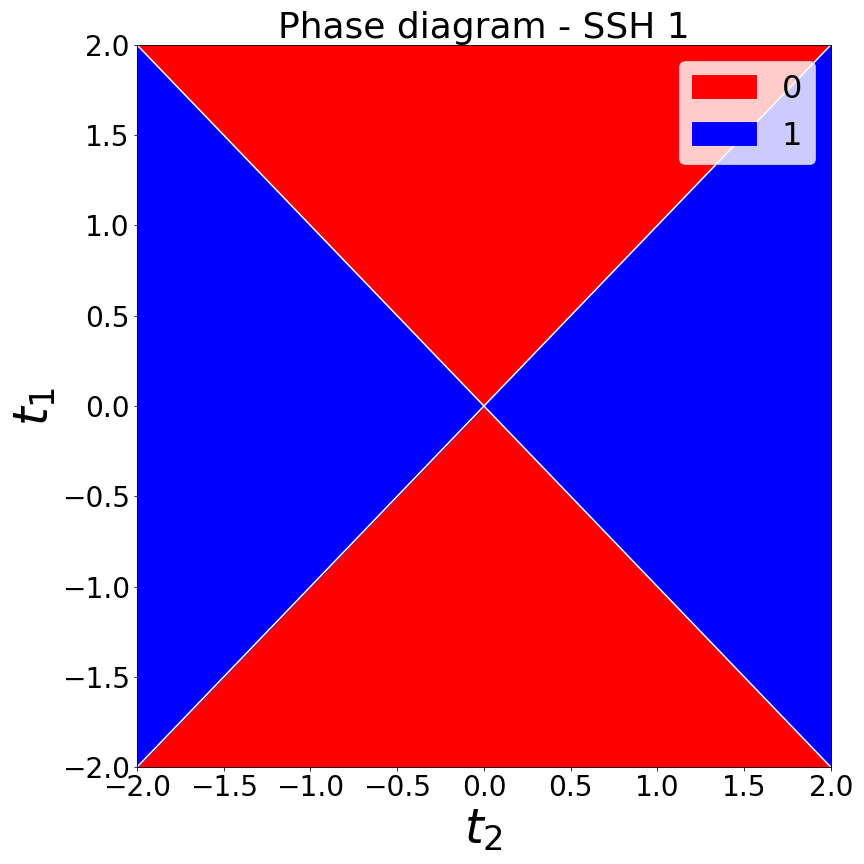
\includegraphics[width=.45\textwidth]{./phase_diagrams/ssh1.png}}\quad
\subfigure[]{\label{ssh2}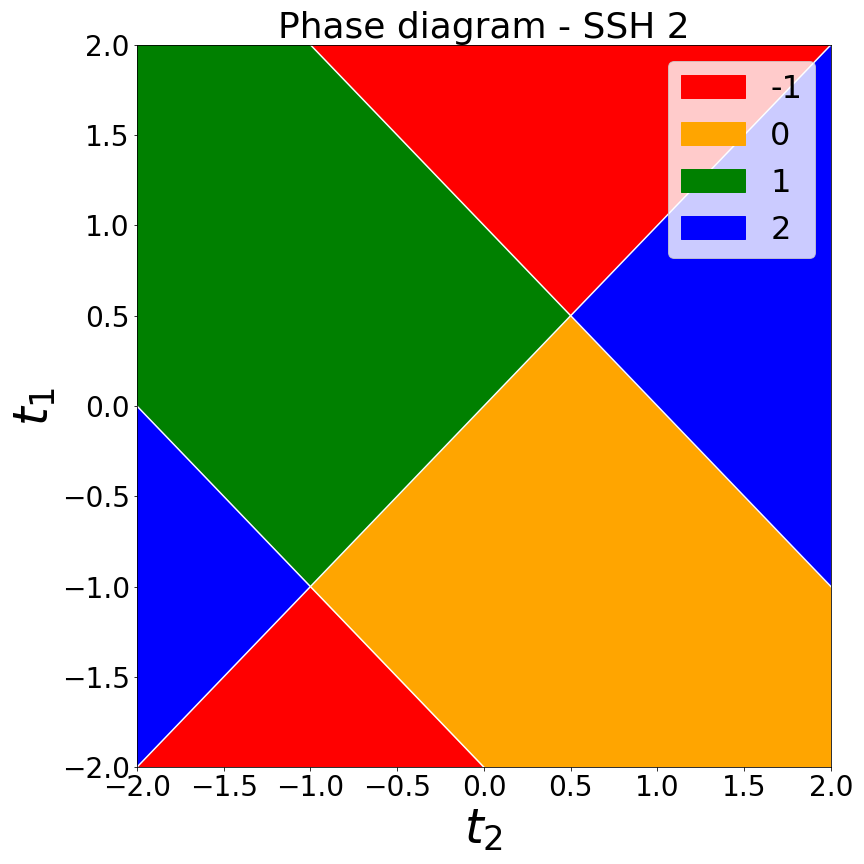
\includegraphics[width=.45\textwidth]{./phase_diagrams/ssh2.png}}
\caption{Phase diagrams in parameter space. a) SSH model with first-neighbor hoppings $t_1$ and $t_2$. The (red) regions with winding number $W$ = 0 are trivial, while the (blue) regions with winding number $W$ = 1 are topologically non-trivial. b) SSH model with first ($t_1$ and $t_2$) and second ($T_1$ and $T_2$) nearest-neighbor hoppings. In this article we set $t_1$ = $t_2$ = 1 and renamed the variables $T_1$ $\rightarrow$ $t_1$, $T_2$ $\rightarrow$ $t_2$ for convenience. The (orange) region with winding number $W$ = 0 is trivial while the others with winding numbers $W$ = -1, $W$ = 1 and $W$ = 2 (red, green and blue respectively) are topologically non-trivial.}
\label{fig:phasediagrams}
\end{figure}

\section*{The eigenvector ensembling algorithm}\citequote{eigenvector_ensembling_alg}

\textcolor{blue}{
We describe here in detail each step of the eigenvector ensembling algorithm as implemented is this article.
\vspace{.3cm}
\begin{enumerate}%[topsep=0pt, partopsep=0pt]
\item[1)] \textbf{Generating Hamiltonians and winding numbers:} we start generating a number of paremeterized Hamiltonians $H(\mathbf{t})$ in real space and their corresponding winding numbers $W(\mathbf{t})$, where $\mathbf{t} = (t_1, t_2,...,t_h)$ is a vector of $h$ hopping parameters (in the simplest case of the SSH model $h$ = 2). These Hamiltonians are $N\times N$ matrices, where $N$ is twice the number of unit cells in the chain.
\item[2)] \textbf{Creating training, validation and test sets:} we split our set of parameterized Hamiltonians and winding numbers into training, validation and test sets, as is usualy done in machine learning. More explicitly, assume our parameter $\mathbf{t}$ takes on the values $\mathbf{t}_1, \mathbf{t}_2, ..., \mathbf{t}_n$ corresponding to the Hamiltonian-winding number pairs ($H_1$, $W_1$), ..., ($H_n$, $W_n$). We partition the set \{($H_i$, $W_i$)$\mid$ $i=1,...,n$\} in three disjoint subsets: the training set, the validation set and the test set.
\item[3)] \textbf{Training on eigenvectors in real space:} since each Hamiltonian $H_i$ is represented by an $N\times N$ matrix, each one will generate $N$ eigenvectors $\mathbf{v}_i^{(1)}, \mathbf{v}_i^{(2)},...,\mathbf{v}_i^{(N)}$. Our supervised learning algorithm of choice will take as inputs the real space eigenvectors $\mathbf{v}^{(j)}_i$ of each Hamiltonian $H_i$ in the training set and be trained to learn the winding number $W_i$ of their parent Hamiltonian $H_i$. Therefore, our dataset will consist of eigenvector-winding number pairs $(\mathbf{v}_i^{(j)}, W_i)$.
\item[4)]\textbf{Eigenvector ensembling:} in order to predict the phase of a system described by a particular Hamiltonian we need to take into account how each of its eigenvectors were classified. This amounts to performing ensemble learning on the eigenvectors of each Hamiltonian. In this work we estimate the phase probabilities for each Hamiltonian as the fraction of its eigenvectors that were classified in each phase.
\item[5)] \textbf{Bootstrapping:} We refine the phase probabilities for each Hamiltonian using a bootstrapping procedure, i.e., we repeat steps (1)-(4) $n_\text{exp}$ times, at each round sampling randomly a new training set from our grid in \textbf{t}-space. The final estimated probabilities are then arrived at by averaging the probabilities obtained in each experiment.
\end{enumerate}
\vspace{.3cm}
In step 3) we used the implementations of decision trees and random forest classifiers from Python's Scikit-learn module. As mentioned in the Introduction, the choice of these particular algorithms is based on their powerful and accessible model explainability capabilities. This choice was made in conformity with our main purpose in this work, which is to exploit model explainability tools to investigate how topological information is distributed along a spatial lattice in SSH systems. Nevertheless, the steps above are flexible and can easily be repurposed for other supervised or unsupervised learning tasks.}\citequote{unsupervised_learning}

\section*{Numerical experiments}

The eigenvector ensembling algorithm consists of five steps: 1) Generating Hamiltonians in real space and their corresponding winding numbers; 2) Creating training, validation and test sets; 3) Training on real space eigenvectors of Hamiltonians in the training set; 4) Eigenvector ensembling and 5) Bootstrapping. A detailed description of the algorithm is found in the section \textbf{The eigenvector ensembling algorithm} in the Supplementary Material. Here we present results of the numerical experiments we performed with it. We start with the results from the simplest case, the SSH model with nearest-neighbor hopping (here called SSH 1, figure \ref{ssh1}), then we analize the SSH model with first and second nearest-neighbor hoppings (here called SSH 2, figure \ref{ssh2}).

In each experiment our grid consisted of 6561 Hamiltonians uniformly distributed in the closed square $[-2,2]\times[-2,2]$ in the $t_1$-$t_2$ plane in parameter space. The goal in each experiment is to recover the corresponding phase diagram in 2D (two-dimensional) parameter space, figures \ref{ssh1} and \ref{ssh2}, from local lattice data in the much higher-dimensional real space (100D - in both experiments lattices have 50 unit cells, yielding 100$\times$100 Hamiltonian matrices).

This task is particularly hard near phase transition boundaries, where numerical computation of winding numbers become less stable. For this reason, when sampling the training set we only consider those Hamiltonians in the grid whose numerically computed winding numbers lie in a range $\epsilon = 0.01$ around the allowed winding number values. Therefore, a good performance metric is the accuracy measured at those Hamiltonians near phase transitions that are never used for training, and thus we assign them to the test set. The remaining Hamiltonians in the grid are split into training and validation sets as detailed in the subsections below.

When generating the Hamiltonians we applied periodic boundary conditions to eliminate border effects. This should make recovering a topological signal from local eigenvector coordinates even harder, since in this case the translational symmetry of the systems should allow for no obvious way to distinguish between unit cells. The choice of periodic boundary conditions also implies that the information recovered from real space data comes from the bulk of the topological systems considered and therefore provides strong evidence for the existence of topological signatures in the bulk of such systems. 

Figures \ref{figexp1_exp} and \ref{figexp2_exp} respectively illustrate single iterations of experiments 1 and 2 as seen from parameter space. The accuracy statistics presented in the following subsections and probability heatmaps shown in figures \ref{ssh1_heatmaps} and \ref{ssh2_heatmaps} were obtained after bootstrapping each experiment $n_{exp}$ = 100 times. The recovered probability heatmaps faithfully portray the phase diagrams in figure \ref{fig:phasediagrams}, with clear phase transition lines appearing in the regions of highest uncertainty.

\subsection*{Experiment 1: Learning a first-neighbor hopping SSH model with decision trees}

Our test set in this experiment contained 1005 Hamiltonians (approx. 15.3\% of all data). Of the remaining 5556 Hamiltonians, 556 were randomly assigned to the training set (approx. 8.5\%) and 5000 (approx. 76.2\%) were used to compute validation scores at each iteration. These proportions between training and validation sets are such that approximately 10\%  of Hamiltonians from outside of the test set were used for training at each iteration. The composition of the train + validation set for this experiment was 50.8\% of Hamiltonians with winding number $W$ = 0 and 49.2\% with winding number $W$ = 1. The composition of the test set was 44.8\% of Hamiltonians with winding number $W$ = 0 and 55.2\% with winding number $W=1$. Our algorithm of choice for this experiment was a simple decision tree model \cite{breiman2017classification}.

The bootstrap allows us to collect several statistics to evaluate performance. In particular, we report mean accuracies on training eigenvectors (98.2\%), validation eigenvectors (96.4\%) and test eigenvectors (78.8\%). Eigenvector ensembling substantially improved mean accuracies for Hamiltonians. These were 100\% for training Hamiltonians, 100\% for validation Hamiltonians and 99.1\% for test Hamiltonians.

The probability heatmaps and phase diagram learned by the combination of decision trees with eigenvector ensembling used in experiment 1 are shown in figure \ref{ssh1_heatmaps}.

\begin{figure}
\centering
\subfigure[]{\label{figexp1_exp:a}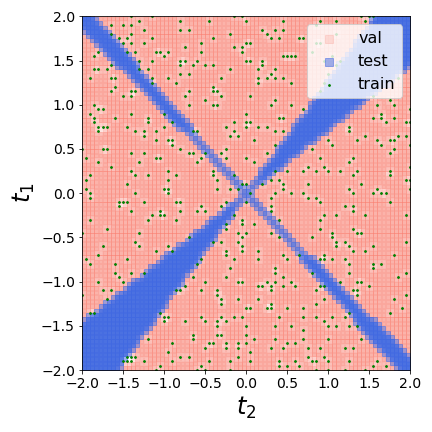
\includegraphics[width=.32\textwidth]{./ssh1/periodic_100_6561/scatter_train_val_test_experiment_0.png}}\quad
\subfigure[]{\label{figexp1_exp:b}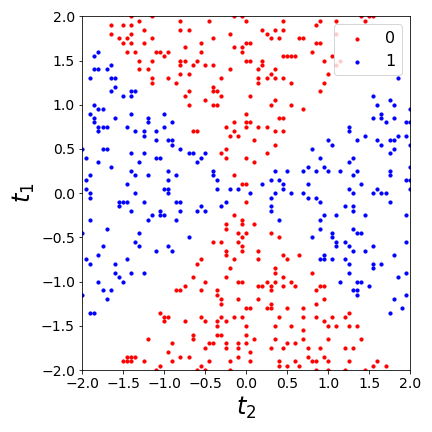
\includegraphics[width=.32\textwidth]{./ssh1/periodic_100_6561/scatter_winding_train_experiment_0.png}}
\subfigure[]{\label{figexp1_exp:c}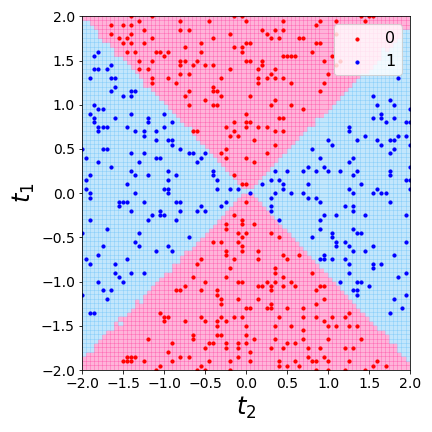
\includegraphics[width=.32\textwidth]{./ssh1/periodic_100_6561/pcolormesh_prediction_grid_experiment_0.png}}
\caption{Visualization of a single iteration of experiment 1 as seen from 2D parameter space. (a) Train/validation/test split. (b) Distribution of winding numbers in the training set. (c) Phase diagram learned from real space lattice data by a combination of decision tree and eigenvector ensembling.}
\label{figexp1_exp}
\end{figure}

\subsection*{Experiment 2: Learning a first- and second-neighbor hoppings SSH model with random forests}
\label{exp2}

This task is considerably more difficult than the previous one due to the higher number of classes and the fact that some of the labels encompass disconnected regions. For this reason, instead of using a single decision tree, we upgraded our model to a random forest \cite{Breiman2001} with 25 decision trees. Our data set consisted of 1040 (15.8\%) test Hamiltonians. The remaining Hamiltonians are randomly split in half between training and validation sets at each iteration, giving 2761 (42.1\%) training Hamiltonians and 2760 (42.1\%) validation Hamiltonians. The distribution of winding numbers for the Hamiltonians in the train + validation set for this experiment was $W$ = -1 (17.9\%), $W$ = 0 (32.5\%), $W$ = 1 (32.3\%) and $W$ = 2 (17.3\%). The distribution of winding numbers for the Hamiltonians in the test set was $W$ = -1 (36.3\%), $W$ = 0 (11.1\%), $W$ = 1 (12.7\%) and $W$ = 2 (39.9\%).

Mean accuracies across 100 repetitions of experiment 2 were 99.9\% for training eigenvectors, 97.1\% for validation eigenvectors and 66.4\% for test eigenvectors. Mean accuracies resulting from eigenvector ensembling were 100\% for training Hamiltonians, 99.7\% for validation Hamiltonians and 88.2\% for test Hamiltonians. The large accuracy gain achieved by eigenvector ensembling in the test set (going from 66.4\% eigenvector accuracy to 88.2\% Hamiltonian accuracy) attests to its power.

The probability heatmaps and phase diagram learned by the combination of random forests with eigenvector ensembling used in experiment 2 are shown in figure \ref{ssh2_heatmaps}.

\begin{figure}
\centering
\subfigure[]{\label{figexp2_exp:a}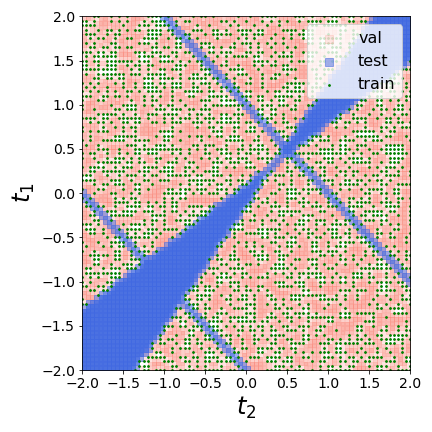
\includegraphics[width=.32\textwidth]{./ssh2/periodic_100_6561/scatter_train_val_test_experiment_0.png}}\quad
\subfigure[]{\label{figexp2_exp:b}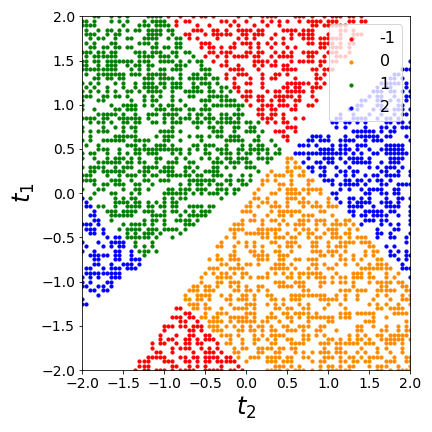
\includegraphics[width=.32\textwidth]{./ssh2/periodic_100_6561/scatter_winding_train_experiment_0.png}}
\subfigure[]{\label{figexp2_exp:c}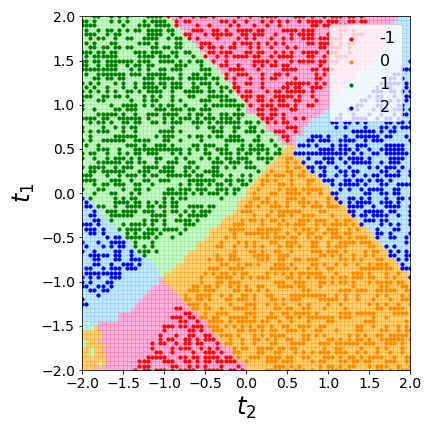
\includegraphics[width=.32\textwidth]{./ssh2/periodic_100_6561/pcolormesh_prediction_grid_experiment_0.png}}
\caption{Visualization of a single iteration of experiment 2 as seen from 2D parameter space. (a) Train/validation/test split. (b) Distribution of winding numbers in the training set. (c) Phase diagram learned from real space lattice data by a combination of random forest and eigenvector ensembling.}
\label{figexp2_exp}
\end{figure}

\section*{Information entropy signatures}

We now analyze how the algorithm was able to recover a global property of the Hamiltonians (their topological phase) from bulk local features (real space eigenvector coordinates on each lattice site). Alongside the fact that decision trees and random forests are very easy to train and visualize, the other reason that led us to test our algorithm with them was that they allow us to check which features (and thus which lattice sites) were most informative in training.

The (normalized) relevance of a feature is given by how much it reduces a loss function (e.g. Shannon information entropy or Gini impurity \cite{friedman2001elements}). By averaging normalized relevances as measured by reduction in the information entropy of ensembles of real space eigenvectors across $n_{exp}$ = 100 iterations of both experiment 1 and experiment 2 we recovered Shannon entropy signals that reveal which lattice sites were consistently more relevant in learning topological phases from data in real space for each experiment. These signals are the information entropy signatures of each topological phase transition. 

The bar plots in figure \ref{feature_importances} show how informative each lattice site was in learning topological phases for experiments 1 and 2. They represent the information entropy signatures along the lattices in each SSH system. For experiment 1, only six lattice sites $S_1$ = (0, 1, 3, 50, 51, 53) corresponding to the two sharp peaks seen in figure \ref{feature_importances_ssh1} contributed approximately 70\% of total reduction in Shannon entropy. Similarly, approximately 30\% of total reduction in the Shannon information entropy of eigenvector data from experiment 2 was achieved by eighteen lattice sites $S_2$ = (0, 1, 2, 3, 4, 5, 46, 48, 49, 50, 51, 53, 94, 95, 96, 97, 98, 99) distributed along the three peaks in figure \ref{feature_importances_ssh2}.

Each of the information entropy signatures shown in figure \ref{feature_importances} captures a general pattern that persists regardless of the length of the lattice (i.e, number of unit cells) used to compute them. They are not, therefore, artifacts of particular choices of hyperparameters used to run the eigenvector ensembling algorithm. We present the information entropy signatures for longer lattices in the section \textbf{Information entropy signatures in the macroscopic limit} in the Supplementary Material.

To see if learning the topological phases can be achieved efficiently by employing simpler models we reran experiments 1 and 2 using only a small subset of most relevant lattice sites. In our rerun of experiment 1 using only lattice sites $S'_1$ = (0, 50, 51, 99) (which contributed approximately 45 \% of total reduction in Shannon information entropy in experiment 1), mean accuracies were 97.0\% for training eigenvectors, 91.5\% for validation eigenvectors and 72.8\% for test eigenvectors. Mean accuracies obtained from eigenvector ensembling were 99.1\% for training Hamiltonians, 99.5\% for validation Hamiltonians and 94.5\% for test Hamiltonians.

Mean accuracies for our rerun of experiment 2 using only lattice sites $S'_2$ = (0, 1, 3, 48, 50, 51, 96, 98, 99) (which contributed approximately 20 \% of total reduction in Shannon information entropy in experiment 2) were 99.9\% for training eigenvectors, 87.7\% for validation eigenvectors and 47.3\% for test eigenvectors. Eigenvector ensembling yields mean accuracies of 100\% for training Hamiltonians, 99.5\% for validation Hamiltonians and 74.5\% for test Hamiltonians.  

These results demonstrate that learning topological phases from local real space data in the bulk is still possible even for small subsets of lattice sites. \textcolor{blue}{In this sense, key topological information can be said to be localized on few sites in the lattice.}\citequote{key_top} We refer the reader to the section \textbf{Learning topological phases from real space data} in the Supplementary Material for a discussion of how this is possible.

\begin{figure}
\centering
\subfigure[]{\label{ssh1_heatmap_0}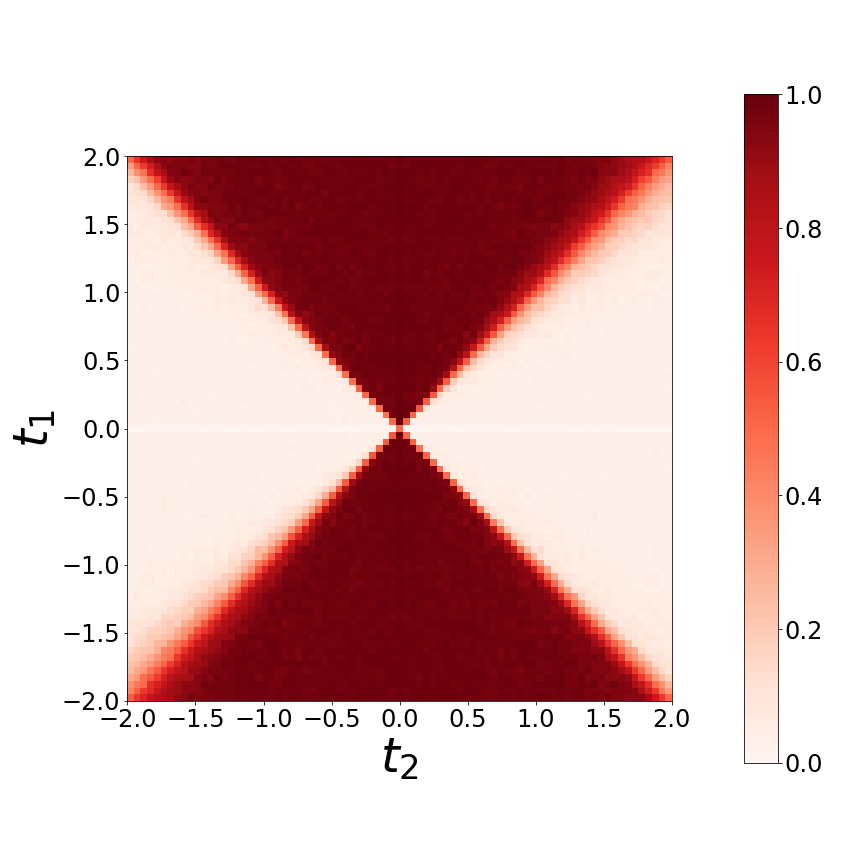
\includegraphics[width=.32\textwidth]{./ssh1/periodic_100_6561/imshow_winding_grid_winding_0_sim.png}}
\subfigure[]{\label{ssh1_heatmap_1}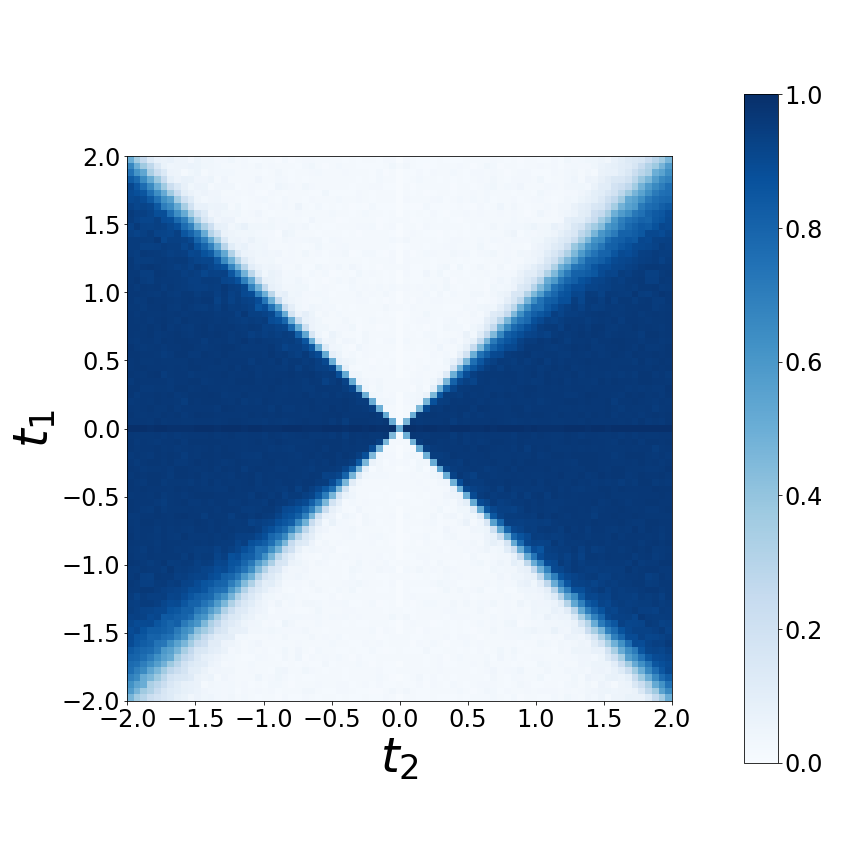
\includegraphics[width=.32\textwidth]{./ssh1/periodic_100_6561/imshow_winding_grid_winding_1_sim.png}}
\subfigure[]{\label{ssh1_heatmap}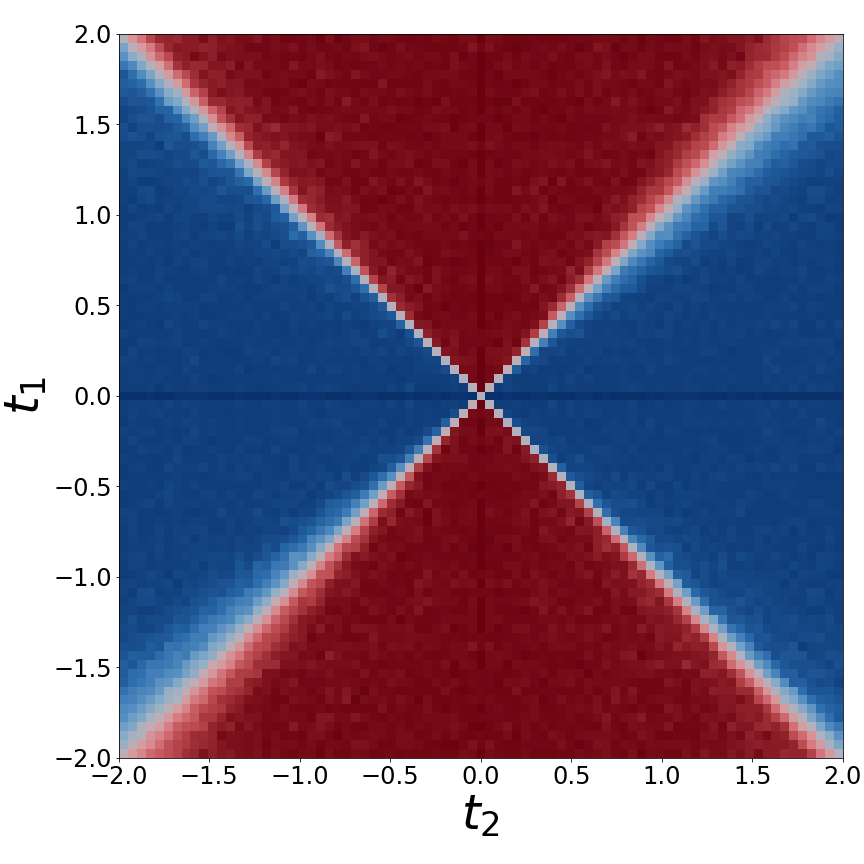
\includegraphics[width=.32\textwidth]{./ssh1/periodic_100_6561/merge_imshow_winding_grids_second_sim.png}}
\caption{Probability heatmaps learned by a combination of decision trees with eigenvector ensembling from bulk real space eigenvector data in experiment 1. Heatmaps were averaged across all 100 iterations of the experiment. (a) Probability heatmap showing the probability that a Hamiltonian in the grid has winding number equal to 0.  (b) Probability heatmap showing the probability that a Hamiltonian in the grid has winding number equal to 1. (c) The phase diagram resulting from heatmaps (a) and (b).}
\label{ssh1_heatmaps}
\end{figure}

\begin{figure}
\centering
\subfigure[]{\label{ssh2_heatmap_-1}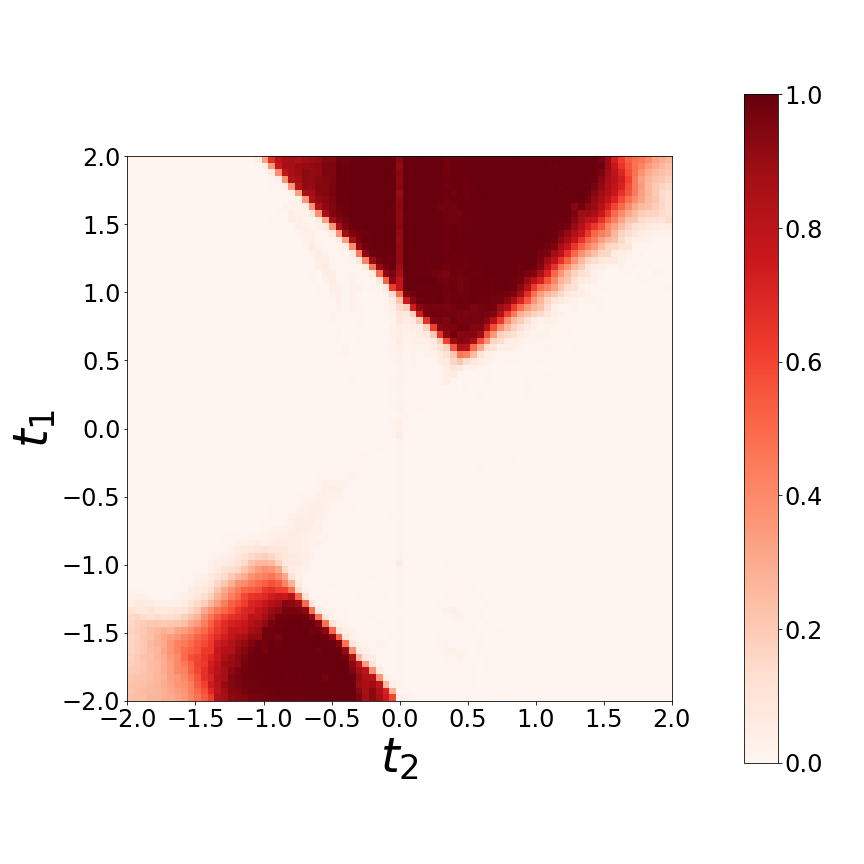
\includegraphics[width=.32\textwidth]{./ssh2/periodic_100_6561/imshow_winding_grid_winding_-1_sim.png}}
\subfigure[]{\label{ssh2_heatmap_0}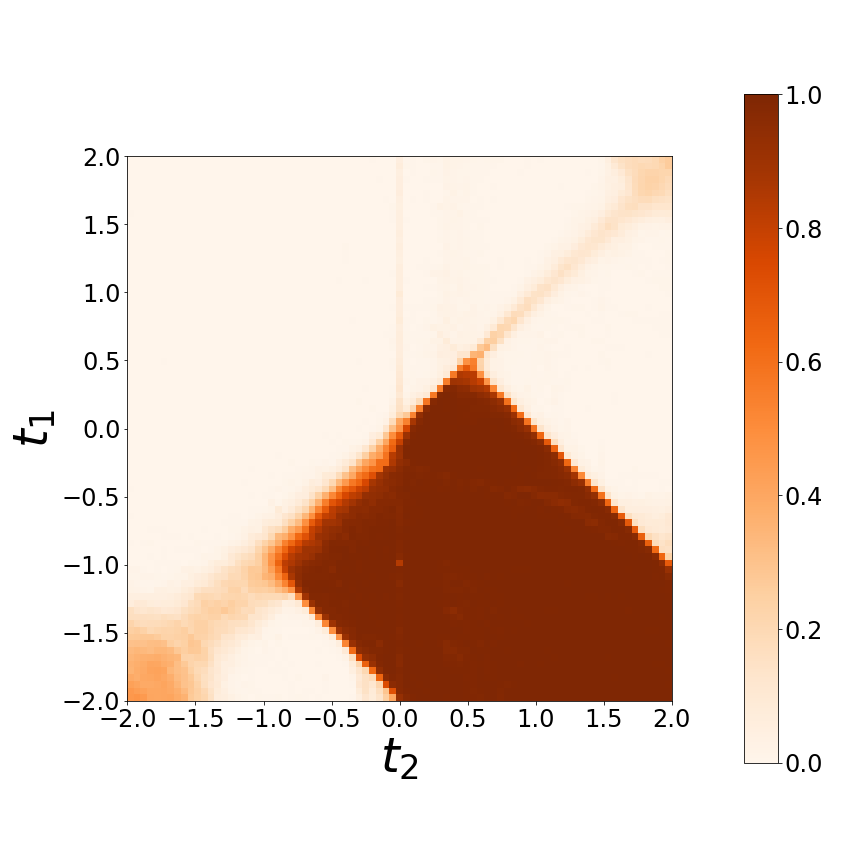
\includegraphics[width=.32\textwidth]{./ssh2/periodic_100_6561/imshow_winding_grid_winding_0_sim.png}}
\subfigure[]{\label{ssh2_heatmap_1}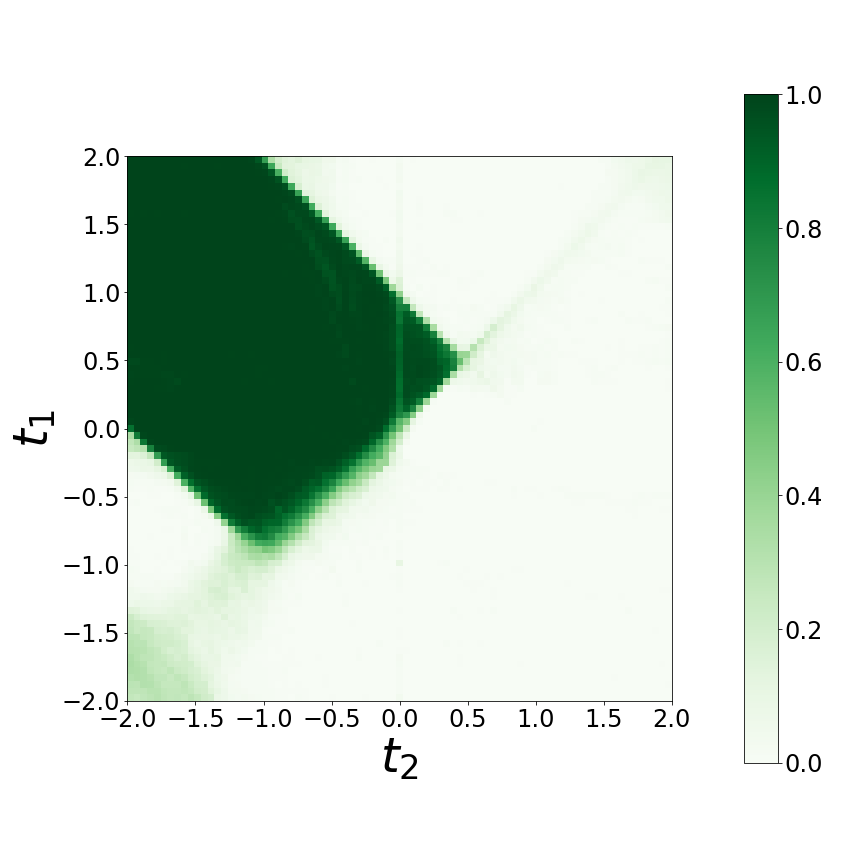
\includegraphics[width=.32\textwidth]{./ssh2/periodic_100_6561/imshow_winding_grid_winding_1_sim.png}}
\subfigure[]{\label{ssh2_heatmap_2}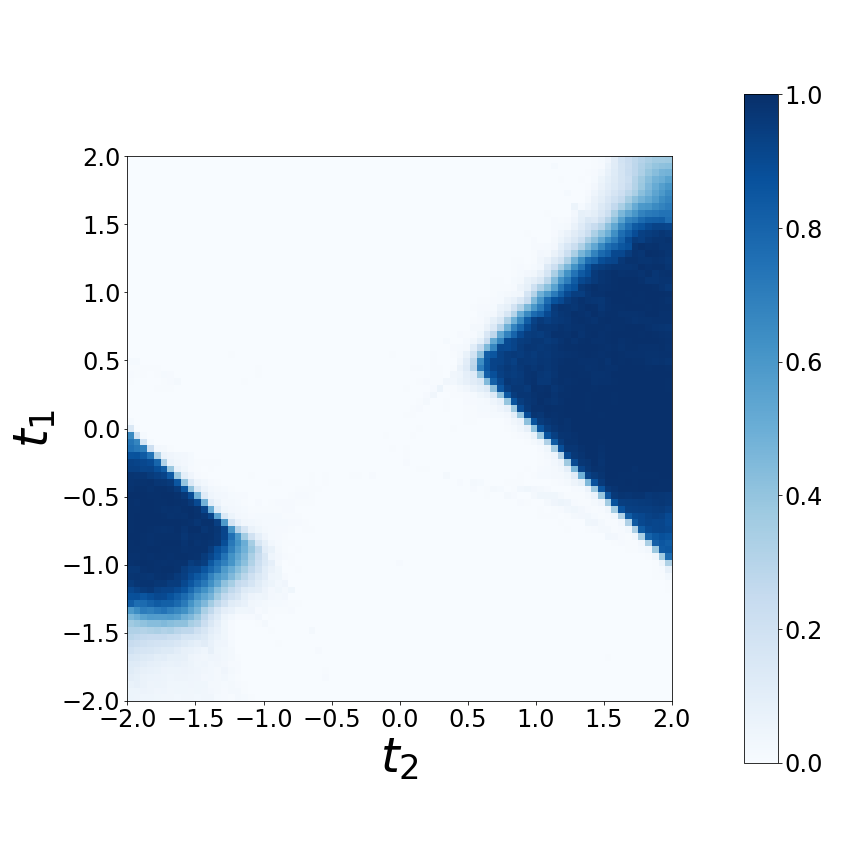
\includegraphics[width=.32\textwidth]{./ssh2/periodic_100_6561/imshow_winding_grid_winding_2_sim.png}}
\subfigure[]{\label{ssh2_heatmap}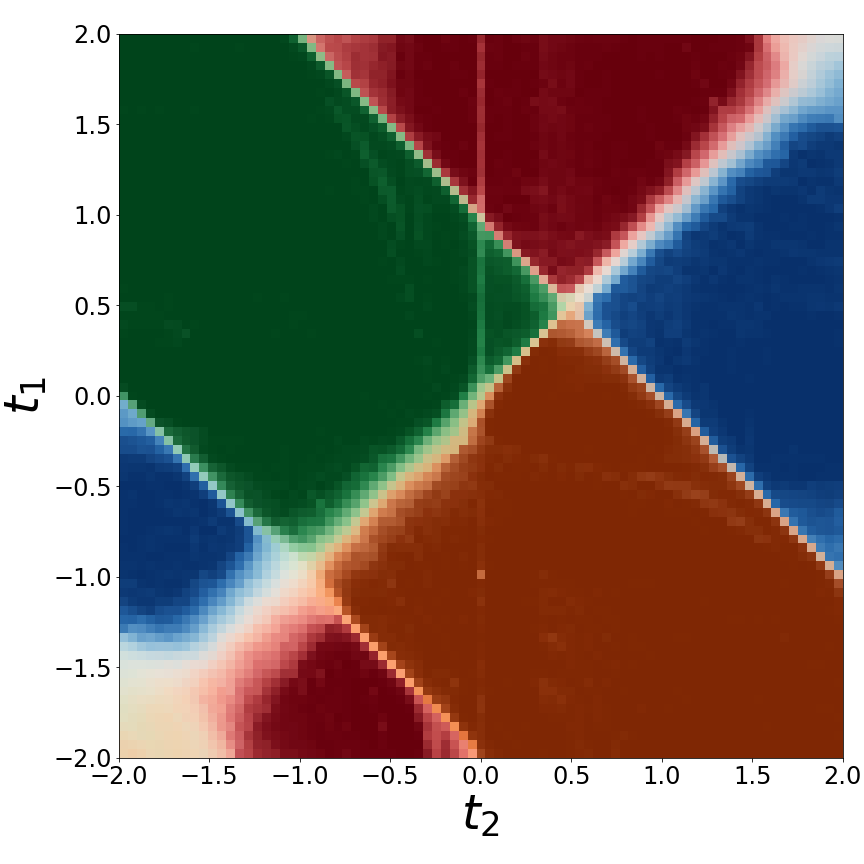
\includegraphics[width=.32\textwidth]{./ssh2/periodic_100_6561/merge_imshow_winding_grids_sim.png}}
\caption{Probability heatmaps learned by a combination of random forests with eigenvector ensembling from bulk real space eigenvector data in experiment 2. Heatmaps were averaged across all 100 iterations of the experiment. (a) Probability heatmap showing the probability that a Hamiltonian in the grid has winding number equal to -1.  (b) Probability heatmap showing the probability that a Hamiltonian in the grid has winding number equal to 0. (c) Probability heatmap showing the probability that a Hamiltonian in the grid has winding number equal to 1. (d) Probability heatmap showing the probability that a Hamiltonian in the grid has winding number equal to 2. (e) The phase diagram resulting from heatmaps (a)-(d).}
\label{ssh2_heatmaps}
\end{figure}

\section*{Discussion}

Given the increasing complexity of systems studied in condensed matter physics and the rising demand for materials with exotic and robust properties to power future technological progress, it is only expected that data-driven approaches to physics will grow in demand. Our work represents a step in this direction, as we have implemented a data-driven approach to the search for new topological materials bypassing the use of wavevector space data.

The development of data-driven methods based on real space lattice data will be particularly relevant to the study of disordered systems in condensed matter. Such systems usually break translational symmetry and therefore are not amenable to wavevector space methods.

An advantage of using data from real space is that it enables us to investigate how topological information is distributed in the system. This was demonstrated by the information entropy signatures recovered from the Shannon entropy of ensembles of eigenvectors in each experiment. The existence of such signals that can be recovered from data from many distinct physical systems but are hard to conceptualize from sheer theoretical reasoning provides a clear example of how machine learning can be an important tool in the investigation and discovery of new quantum materials.

We should remark on the subtleties of the information entropy signatures presented here. Although they give us a visualization of how important each lattice site was in determining the topological phases of Hamiltonians, these importances actually express a global property of the whole lattice. Therefore, a lattice site that appears unimportant in an information entropy signature plot may not be unimportant or void of topological information by itself. To give a concrete example, reduction in Shannon entropy tends to be distributed among highly correlated variables. This implies that if only a single lattice site in a highly correlated subset is used, it will likely inherit most of the reduction in Shannon entropy from the other correlated lattice sites in the subset. In this regard the information entropy signatures presented here express a summary of relations between lattice sites and are therefore intrinsically global. Furthermore, it should be emphasized that these signals were recovered from the analysis of data from several thousand SSH systems in each experiment and therefore they are not a property of a single SSH lattice. They are rather a pattern that emerges from correlating topological phase with lattice eigenvector data for several SSH systems.   

We performed several tests on the information entropy signatures. By rerunning each experiment with longer lattices (i.e. increasing the number of unit cells) we have verified that the signals in figures \ref{feature_importances_ssh1} and \ref{feature_importances_ssh2} appear to converge to well defined continuous density functions in the macroscopic limit. The macroscopic limit of these information entropy signals may be an important signature of topological systems and thus merits further theoretical investigation. A detailed discussion of this point is presented in the section \textbf{Information entropy signatures in the macroscopic limit} in the Supplementary Material.

Recent works have demonstrated the existence of local topological markers in real space that carry important information on the topological state of a system \cite{PhysRevB.84.241106,caio2019topological}.  Given that topological signals such as the ones shown in figures \ref{feature_importances_ssh1} and \ref{feature_importances_ssh2} are measured in terms of quantities that have actual physical meaning such as Shannon information entropy or Gini impurity, the results presented here suggest a new road for theoretical investigation. Whether there is any relationship between local topological markers and the information entropy of the ensemble of eigenvectors is left for speculation.

The eigenvector ensembling algorithm employed in this work is likely to have further applications in data-driven physics. This is because most of physics is based on eigenvector decomposition, and statistical physics itself can be seen as an application of similar ensembling principles. 

\textcolor{blue}{As a concrete example, the study of several many-body systems of current interest in condensed matter physics is hindered by their large dimensionality. This problem, known as \emph{the curse of dimensionality} in the scientific computing community, arises from the necessity of collecting or processing exponentially larger amounts of data as the feature space dimensionality of a problem grows. An approach based on eigenvector ensembling can be of use in such situations both as a dimensionality reduction tool and as a sampling strategy. The first case was illustrated in this work, where it was shown that relevant topological information of SSH systems can be retrieved from few sites in a lattice, which can be exploited as a dimensionality reduction strategy. The latter case, which was not explored here, also poses interesting possibilities, such as sampling eigenstates according to a desired distribution in Monte Carlo simulations of condensed matter systems. Indeed, sampling eigenvectors from a carefully designed probability distribution can ultimately lead to a great reduction in the dimensionality of a problem while still capturing all the relevant physics of a system.}\citequote{pipeline_not_work}  We therefore expect that a much broader class of data-driven physics problems could benefit from the techniques described in this paper.

One final comment should be made about the flourishing relationship between physics and machine learning. In this work we have demonstrated how a machine learning approach can provide new insights into complex physical phenomena of current interest. The other direction of this relationship (physics enhancing understanding in machine learning) is equally important. As the need for ever more powerful machine learning algorithms continues to grow, the development of mathematical frameworks for understanding general data spaces (i.e., a physics of data) will be of crucial relevance. This pursuit is seen in many theoretical works investigating the intriguing connections between geometry, topology and data \cite{carlsson2009topology}$^-$\cite{belkin2003problems}. The detailed study of data generated by physical models with non-trivial geometrical and topological properties such as the SSH model may provide invaluable insights into the structure and shape of real world high-dimensional data, since these models usually underscore well known mathematical frameworks behind the data generating process, a feature that is often absent from machine learning applications. Thus, far from being restricted to applications in physics, the study of the topological and geometrical properties of data sets generated by physical models will also be of great value to the machine learning and artificial intelligence communities.  

\begin{figure}
\centering
\subfigure[]{\label{feature_importances_ssh1}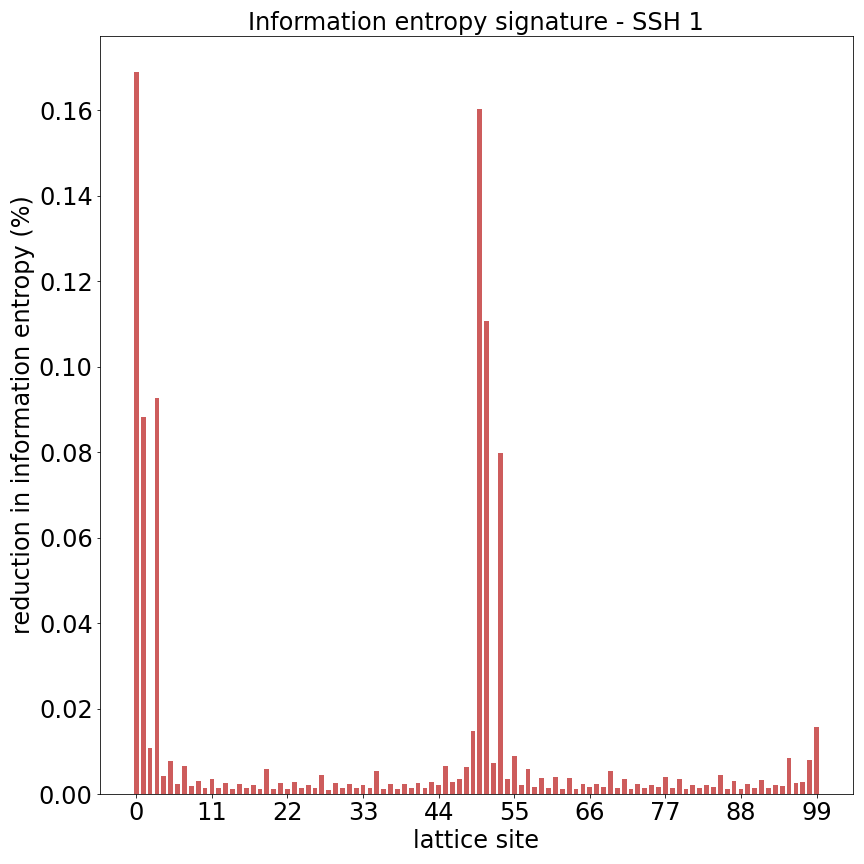
\includegraphics[width=0.49\textwidth]{./ssh1/periodic_100_6561/plot_feature_importances.png}}\quad
\subfigure[]{\label{feature_importances_ssh2}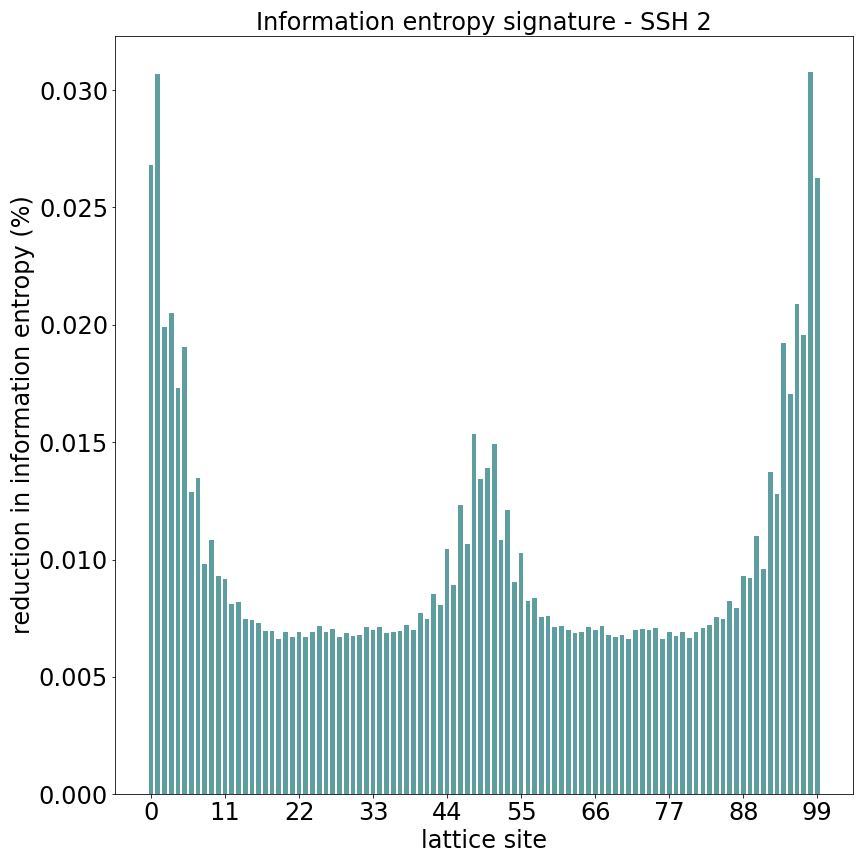
\includegraphics[width=0.49\textwidth]{./ssh2/periodic_100_6561/plot_feature_importances.png}}\quad
\caption{Information entropy signatures of the topological phase transitions from experiments 1 and 2. (a) In experiment 1, the two sharp peaks in the Shannon entropy signal account for approximately 70\% of reduction in information entropy. These two peaks correspond to the lattice sites $S_1$. (b) In experiment 2, the three visible peaks account for approximately 30\% of reduction in information entropy. These three peaks are located along lattice sites $S_2$.}
\label{feature_importances}
\end{figure}

\citequote{motif_real_space}

%merlin.mbs apsrev4-1.bst 2010-07-25 4.21a (PWD, AO, DPC) hacked
%Control: key (0)
%Control: author (8) initials jnrlst
%Control: editor formatted (1) identically to author
%Control: production of article title (-1) disabled
%Control: page (0) single
%Control: year (1) truncated
%Control: production of eprint (0) enabled
\begin{thebibliography}{56}%
\makeatletter
\providecommand \@ifxundefined [1]{%
 \@ifx{#1\undefined}
}%
\providecommand \@ifnum [1]{%
 \ifnum #1\expandafter \@firstoftwo
 \else \expandafter \@secondoftwo
 \fi
}%
\providecommand \@ifx [1]{%
 \ifx #1\expandafter \@firstoftwo
 \else \expandafter \@secondoftwo
 \fi
}%
\providecommand \natexlab [1]{#1}%
\providecommand \enquote  [1]{``#1''}%
\providecommand \bibnamefont  [1]{#1}%
\providecommand \bibfnamefont [1]{#1}%
\providecommand \citenamefont [1]{#1}%
\providecommand \href@noop [0]{\@secondoftwo}%
\providecommand \href [0]{\begingroup \@sanitize@url \@href}%
\providecommand \@href[1]{\@@startlink{#1}\@@href}%
\providecommand \@@href[1]{\endgroup#1\@@endlink}%
\providecommand \@sanitize@url [0]{\catcode `\\12\catcode `\$12\catcode
  `\&12\catcode `\#12\catcode `\^12\catcode `\_12\catcode `\%12\relax}%
\providecommand \@@startlink[1]{}%
\providecommand \@@endlink[0]{}%
\providecommand \url  [0]{\begingroup\@sanitize@url \@url }%
\providecommand \@url [1]{\endgroup\@href {#1}{\urlprefix }}%
\providecommand \urlprefix  [0]{URL }%
\providecommand \Eprint [0]{\href }%
\providecommand \doibase [0]{http://dx.doi.org/}%
\providecommand \selectlanguage [0]{\@gobble}%
\providecommand \bibinfo  [0]{\@secondoftwo}%
\providecommand \bibfield  [0]{\@secondoftwo}%
\providecommand \translation [1]{[#1]}%
\providecommand \BibitemOpen [0]{}%
\providecommand \bibitemStop [0]{}%
\providecommand \bibitemNoStop [0]{.\EOS\space}%
\providecommand \EOS [0]{\spacefactor3000\relax}%
\providecommand \BibitemShut  [1]{\csname bibitem#1\endcsname}%
\let\auto@bib@innerbib\@empty
%</preamble>
\bibitem [{\citenamefont {Hasan}\ and\ \citenamefont
  {Kane}(2010)}]{RevModPhys.82.3045}%
  \BibitemOpen
  \bibfield  {author} {\bibinfo {author} {\bibfnamefont {M.~Z.}\ \bibnamefont
  {Hasan}}\ and\ \bibinfo {author} {\bibfnamefont {C.~L.}\ \bibnamefont
  {Kane}},\ }\href@noop {} {\bibfield  {journal} {\bibinfo  {journal} {Rev.
  Mod. Phys.}\ }\textbf {\bibinfo {volume} {82}},\ \bibinfo {pages} {3045}
  (\bibinfo {year} {2010})}\BibitemShut {NoStop}%
\bibitem [{\citenamefont {Continentino}(2017)}]{CONTINENTINO2017A1}%
  \BibitemOpen
  \bibfield  {author} {\bibinfo {author} {\bibfnamefont {M.~A.}\ \bibnamefont
  {Continentino}},\ }\href@noop {} {\bibfield  {journal} {\bibinfo  {journal}
  {Physica B: Condensed Matter}\ }\textbf {\bibinfo {volume} {505}},\ \bibinfo
  {pages} {A1 } (\bibinfo {year} {2017})}\BibitemShut {NoStop}%
\bibitem [{\citenamefont {Puel}\ \emph {et~al.}(2017)\citenamefont {Puel},
  \citenamefont {Sacramento},\ and\ \citenamefont
  {Continentino}}]{PhysRevB.95.094509}%
  \BibitemOpen
  \bibfield  {author} {\bibinfo {author} {\bibfnamefont {T.~O.}\ \bibnamefont
  {Puel}}, \bibinfo {author} {\bibfnamefont {P.~D.}\ \bibnamefont
  {Sacramento}}, \ and\ \bibinfo {author} {\bibfnamefont {M.~A.}\ \bibnamefont
  {Continentino}},\ }\href@noop {} {\bibfield  {journal} {\bibinfo  {journal}
  {Phys. Rev. B}\ }\textbf {\bibinfo {volume} {95}},\ \bibinfo {pages} {094509}
  (\bibinfo {year} {2017})}\BibitemShut {NoStop}%
\bibitem [{\citenamefont {Griffith}\ and\ \citenamefont
  {Continentino}(2018)}]{PhysRevE.97.012107}%
  \BibitemOpen
  \bibfield  {author} {\bibinfo {author} {\bibfnamefont {M.~A.}\ \bibnamefont
  {Griffith}}\ and\ \bibinfo {author} {\bibfnamefont {M.~A.}\ \bibnamefont
  {Continentino}},\ }\href@noop {} {\bibfield  {journal} {\bibinfo  {journal}
  {Phys. Rev. E}\ }\textbf {\bibinfo {volume} {97}},\ \bibinfo {pages} {012107}
  (\bibinfo {year} {2018})}\BibitemShut {NoStop}%
\bibitem [{\citenamefont {Ryu}\ \emph {et~al.}(2010)\citenamefont {Ryu},
  \citenamefont {Schnyder}, \citenamefont {Furusaki},\ and\ \citenamefont
  {Ludwig}}]{ryu2010topological}%
  \BibitemOpen
  \bibfield  {author} {\bibinfo {author} {\bibfnamefont {S.}~\bibnamefont
  {Ryu}}, \bibinfo {author} {\bibfnamefont {A.~P.}\ \bibnamefont {Schnyder}},
  \bibinfo {author} {\bibfnamefont {A.}~\bibnamefont {Furusaki}}, \ and\
  \bibinfo {author} {\bibfnamefont {A.~W.}\ \bibnamefont {Ludwig}},\
  }\href@noop {} {\bibfield  {journal} {\bibinfo  {journal} {New Journal of
  Physics}\ }\textbf {\bibinfo {volume} {12}},\ \bibinfo {pages} {065010}
  (\bibinfo {year} {2010})}\BibitemShut {NoStop}%
\bibitem [{\citenamefont {Atala}\ \emph {et~al.}(2013)\citenamefont {Atala},
  \citenamefont {Aidelsburger}, \citenamefont {Barreiro}, \citenamefont
  {Abanin}, \citenamefont {Kitagawa}, \citenamefont {Demler},\ and\
  \citenamefont {Bloch}}]{atala2013direct}%
  \BibitemOpen
  \bibfield  {author} {\bibinfo {author} {\bibfnamefont {M.}~\bibnamefont
  {Atala}}, \bibinfo {author} {\bibfnamefont {M.}~\bibnamefont {Aidelsburger}},
  \bibinfo {author} {\bibfnamefont {J.~T.}\ \bibnamefont {Barreiro}}, \bibinfo
  {author} {\bibfnamefont {D.}~\bibnamefont {Abanin}}, \bibinfo {author}
  {\bibfnamefont {T.}~\bibnamefont {Kitagawa}}, \bibinfo {author}
  {\bibfnamefont {E.}~\bibnamefont {Demler}}, \ and\ \bibinfo {author}
  {\bibfnamefont {I.}~\bibnamefont {Bloch}},\ }\href@noop {} {\bibfield
  {journal} {\bibinfo  {journal} {Nature Physics}\ }\textbf {\bibinfo {volume}
  {9}},\ \bibinfo {pages} {795} (\bibinfo {year} {2013})}\BibitemShut {NoStop}%
\bibitem [{\citenamefont {Stuhl}\ \emph {et~al.}(2015)\citenamefont {Stuhl},
  \citenamefont {Lu}, \citenamefont {Aycock}, \citenamefont {Genkina},\ and\
  \citenamefont {Spielman}}]{Stuhl1514}%
  \BibitemOpen
  \bibfield  {author} {\bibinfo {author} {\bibfnamefont {B.~K.}\ \bibnamefont
  {Stuhl}}, \bibinfo {author} {\bibfnamefont {H.-I.}\ \bibnamefont {Lu}},
  \bibinfo {author} {\bibfnamefont {L.~M.}\ \bibnamefont {Aycock}}, \bibinfo
  {author} {\bibfnamefont {D.}~\bibnamefont {Genkina}}, \ and\ \bibinfo
  {author} {\bibfnamefont {I.~B.}\ \bibnamefont {Spielman}},\ }\href@noop {}
  {\bibfield  {journal} {\bibinfo  {journal} {Science}\ }\textbf {\bibinfo
  {volume} {349}},\ \bibinfo {pages} {1514} (\bibinfo {year}
  {2015})}\BibitemShut {NoStop}%
\bibitem [{\citenamefont {Leder}\ \emph {et~al.}(2016)\citenamefont {Leder},
  \citenamefont {Grossert}, \citenamefont {Sitta}, \citenamefont {Genske},
  \citenamefont {Rosch},\ and\ \citenamefont {Weitz}}]{leder2016real}%
  \BibitemOpen
  \bibfield  {author} {\bibinfo {author} {\bibfnamefont {M.}~\bibnamefont
  {Leder}}, \bibinfo {author} {\bibfnamefont {C.}~\bibnamefont {Grossert}},
  \bibinfo {author} {\bibfnamefont {L.}~\bibnamefont {Sitta}}, \bibinfo
  {author} {\bibfnamefont {M.}~\bibnamefont {Genske}}, \bibinfo {author}
  {\bibfnamefont {A.}~\bibnamefont {Rosch}}, \ and\ \bibinfo {author}
  {\bibfnamefont {M.}~\bibnamefont {Weitz}},\ }\href@noop {} {\bibfield
  {journal} {\bibinfo  {journal} {Nature communications}\ }\textbf {\bibinfo
  {volume} {7}},\ \bibinfo {pages} {13112} (\bibinfo {year}
  {2016})}\BibitemShut {NoStop}%
\bibitem [{\citenamefont {Goldman}\ \emph {et~al.}(2016)\citenamefont
  {Goldman}, \citenamefont {Budich},\ and\ \citenamefont
  {Zoller}}]{goldman2016topological}%
  \BibitemOpen
  \bibfield  {author} {\bibinfo {author} {\bibfnamefont {N.}~\bibnamefont
  {Goldman}}, \bibinfo {author} {\bibfnamefont {J.}~\bibnamefont {Budich}}, \
  and\ \bibinfo {author} {\bibfnamefont {P.}~\bibnamefont {Zoller}},\
  }\href@noop {} {\bibfield  {journal} {\bibinfo  {journal} {Nature Physics}\
  }\textbf {\bibinfo {volume} {12}},\ \bibinfo {pages} {639} (\bibinfo {year}
  {2016})}\BibitemShut {NoStop}%
\bibitem [{\citenamefont {Meier}\ \emph {et~al.}(2016)\citenamefont {Meier},
  \citenamefont {An},\ and\ \citenamefont {Gadway}}]{meier2016observation}%
  \BibitemOpen
  \bibfield  {author} {\bibinfo {author} {\bibfnamefont {E.~J.}\ \bibnamefont
  {Meier}}, \bibinfo {author} {\bibfnamefont {F.~A.}\ \bibnamefont {An}}, \
  and\ \bibinfo {author} {\bibfnamefont {B.}~\bibnamefont {Gadway}},\
  }\href@noop {} {\bibfield  {journal} {\bibinfo  {journal} {Nature
  communications}\ }\textbf {\bibinfo {volume} {7}},\ \bibinfo {pages} {13986}
  (\bibinfo {year} {2016})}\BibitemShut {NoStop}%
\bibitem [{\citenamefont {Hafezi}\ \emph {et~al.}(2013)\citenamefont {Hafezi},
  \citenamefont {Mittal}, \citenamefont {Fan}, \citenamefont {Migdall},\ and\
  \citenamefont {Taylor}}]{hafezi2013imaging}%
  \BibitemOpen
  \bibfield  {author} {\bibinfo {author} {\bibfnamefont {M.}~\bibnamefont
  {Hafezi}}, \bibinfo {author} {\bibfnamefont {S.}~\bibnamefont {Mittal}},
  \bibinfo {author} {\bibfnamefont {J.}~\bibnamefont {Fan}}, \bibinfo {author}
  {\bibfnamefont {A.}~\bibnamefont {Migdall}}, \ and\ \bibinfo {author}
  {\bibfnamefont {J.}~\bibnamefont {Taylor}},\ }\href@noop {} {\bibfield
  {journal} {\bibinfo  {journal} {Nature Photonics}\ }\textbf {\bibinfo
  {volume} {7}},\ \bibinfo {pages} {1001} (\bibinfo {year} {2013})}\BibitemShut
  {NoStop}%
\bibitem [{\citenamefont {Lu}\ \emph {et~al.}(2016)\citenamefont {Lu},
  \citenamefont {Joannopoulos},\ and\ \citenamefont
  {Solja{\v{c}}i{\'c}}}]{lu2016topological}%
  \BibitemOpen
  \bibfield  {author} {\bibinfo {author} {\bibfnamefont {L.}~\bibnamefont
  {Lu}}, \bibinfo {author} {\bibfnamefont {J.~D.}\ \bibnamefont
  {Joannopoulos}}, \ and\ \bibinfo {author} {\bibfnamefont {M.}~\bibnamefont
  {Solja{\v{c}}i{\'c}}},\ }\href@noop {} {\bibfield  {journal} {\bibinfo
  {journal} {Nature Physics}\ }\textbf {\bibinfo {volume} {12}},\ \bibinfo
  {pages} {626} (\bibinfo {year} {2016})}\BibitemShut {NoStop}%
\bibitem [{\citenamefont {Peano}\ \emph {et~al.}(2015)\citenamefont {Peano},
  \citenamefont {Brendel}, \citenamefont {Schmidt},\ and\ \citenamefont
  {Marquardt}}]{PhysRevX.5.031011}%
  \BibitemOpen
  \bibfield  {author} {\bibinfo {author} {\bibfnamefont {V.}~\bibnamefont
  {Peano}}, \bibinfo {author} {\bibfnamefont {C.}~\bibnamefont {Brendel}},
  \bibinfo {author} {\bibfnamefont {M.}~\bibnamefont {Schmidt}}, \ and\
  \bibinfo {author} {\bibfnamefont {F.}~\bibnamefont {Marquardt}},\ }\href@noop
  {} {\bibfield  {journal} {\bibinfo  {journal} {Phys. Rev. X}\ }\textbf
  {\bibinfo {volume} {5}},\ \bibinfo {pages} {031011} (\bibinfo {year}
  {2015})}\BibitemShut {NoStop}%
\bibitem [{\citenamefont {Kitagawa}\ \emph {et~al.}(2012)\citenamefont
  {Kitagawa}, \citenamefont {Broome}, \citenamefont {Fedrizzi}, \citenamefont
  {Rudner}, \citenamefont {Berg}, \citenamefont {Kassal}, \citenamefont
  {Aspuru-Guzik}, \citenamefont {Demler},\ and\ \citenamefont
  {White}}]{kitagawa2012observation}%
  \BibitemOpen
  \bibfield  {author} {\bibinfo {author} {\bibfnamefont {T.}~\bibnamefont
  {Kitagawa}}, \bibinfo {author} {\bibfnamefont {M.~A.}\ \bibnamefont
  {Broome}}, \bibinfo {author} {\bibfnamefont {A.}~\bibnamefont {Fedrizzi}},
  \bibinfo {author} {\bibfnamefont {M.~S.}\ \bibnamefont {Rudner}}, \bibinfo
  {author} {\bibfnamefont {E.}~\bibnamefont {Berg}}, \bibinfo {author}
  {\bibfnamefont {I.}~\bibnamefont {Kassal}}, \bibinfo {author} {\bibfnamefont
  {A.}~\bibnamefont {Aspuru-Guzik}}, \bibinfo {author} {\bibfnamefont
  {E.}~\bibnamefont {Demler}}, \ and\ \bibinfo {author} {\bibfnamefont {A.~G.}\
  \bibnamefont {White}},\ }\href@noop {} {\bibfield  {journal} {\bibinfo
  {journal} {Nature communications}\ }\textbf {\bibinfo {volume} {3}},\
  \bibinfo {pages} {882} (\bibinfo {year} {2012})}\BibitemShut {NoStop}%
\bibitem [{\citenamefont {Cardano}\ \emph {et~al.}(2016)\citenamefont
  {Cardano}, \citenamefont {Maffei}, \citenamefont {Massa}, \citenamefont
  {Piccirillo}, \citenamefont {De~Lisio}, \citenamefont {De~Filippis},
  \citenamefont {Cataudella}, \citenamefont {Santamato},\ and\ \citenamefont
  {Marrucci}}]{cardano2016statistical}%
  \BibitemOpen
  \bibfield  {author} {\bibinfo {author} {\bibfnamefont {F.}~\bibnamefont
  {Cardano}}, \bibinfo {author} {\bibfnamefont {M.}~\bibnamefont {Maffei}},
  \bibinfo {author} {\bibfnamefont {F.}~\bibnamefont {Massa}}, \bibinfo
  {author} {\bibfnamefont {B.}~\bibnamefont {Piccirillo}}, \bibinfo {author}
  {\bibfnamefont {C.}~\bibnamefont {De~Lisio}}, \bibinfo {author}
  {\bibfnamefont {G.}~\bibnamefont {De~Filippis}}, \bibinfo {author}
  {\bibfnamefont {V.}~\bibnamefont {Cataudella}}, \bibinfo {author}
  {\bibfnamefont {E.}~\bibnamefont {Santamato}}, \ and\ \bibinfo {author}
  {\bibfnamefont {L.}~\bibnamefont {Marrucci}},\ }\href@noop {} {\bibfield
  {journal} {\bibinfo  {journal} {Nature communications}\ }\textbf {\bibinfo
  {volume} {7}},\ \bibinfo {pages} {11439} (\bibinfo {year}
  {2016})}\BibitemShut {NoStop}%
\bibitem [{\citenamefont {Flurin}\ \emph {et~al.}(2017)\citenamefont {Flurin},
  \citenamefont {Ramasesh}, \citenamefont {Hacohen-Gourgy}, \citenamefont
  {Martin}, \citenamefont {Yao},\ and\ \citenamefont
  {Siddiqi}}]{PhysRevX.7.031023}%
  \BibitemOpen
  \bibfield  {author} {\bibinfo {author} {\bibfnamefont {E.}~\bibnamefont
  {Flurin}}, \bibinfo {author} {\bibfnamefont {V.~V.}\ \bibnamefont
  {Ramasesh}}, \bibinfo {author} {\bibfnamefont {S.}~\bibnamefont
  {Hacohen-Gourgy}}, \bibinfo {author} {\bibfnamefont {L.~S.}\ \bibnamefont
  {Martin}}, \bibinfo {author} {\bibfnamefont {N.~Y.}\ \bibnamefont {Yao}}, \
  and\ \bibinfo {author} {\bibfnamefont {I.}~\bibnamefont {Siddiqi}},\
  }\href@noop {} {\bibfield  {journal} {\bibinfo  {journal} {Phys. Rev. X}\
  }\textbf {\bibinfo {volume} {7}},\ \bibinfo {pages} {031023} (\bibinfo {year}
  {2017})}\BibitemShut {NoStop}%
\bibitem [{\citenamefont {Soluyanov}\ \emph {et~al.}(2015)\citenamefont
  {Soluyanov}, \citenamefont {Gresch}, \citenamefont {Wang}, \citenamefont
  {Wu}, \citenamefont {Troyer}, \citenamefont {Dai},\ and\ \citenamefont
  {Bernevig}}]{soluyanov2015type}%
  \BibitemOpen
  \bibfield  {author} {\bibinfo {author} {\bibfnamefont {A.~A.}\ \bibnamefont
  {Soluyanov}}, \bibinfo {author} {\bibfnamefont {D.}~\bibnamefont {Gresch}},
  \bibinfo {author} {\bibfnamefont {Z.}~\bibnamefont {Wang}}, \bibinfo {author}
  {\bibfnamefont {Q.}~\bibnamefont {Wu}}, \bibinfo {author} {\bibfnamefont
  {M.}~\bibnamefont {Troyer}}, \bibinfo {author} {\bibfnamefont
  {X.}~\bibnamefont {Dai}}, \ and\ \bibinfo {author} {\bibfnamefont {B.~A.}\
  \bibnamefont {Bernevig}},\ }\href@noop {} {\bibfield  {journal} {\bibinfo
  {journal} {Nature}\ }\textbf {\bibinfo {volume} {527}},\ \bibinfo {pages}
  {495} (\bibinfo {year} {2015})}\BibitemShut {NoStop}%
\bibitem [{\citenamefont {Lv}\ \emph {et~al.}(2015)\citenamefont {Lv},
  \citenamefont {Weng}, \citenamefont {Fu}, \citenamefont {Wang}, \citenamefont
  {Miao}, \citenamefont {Ma}, \citenamefont {Richard}, \citenamefont {Huang},
  \citenamefont {Zhao}, \citenamefont {Chen}, \citenamefont {Fang},
  \citenamefont {Dai}, \citenamefont {Qian},\ and\ \citenamefont
  {Ding}}]{PhysRevX.5.031013}%
  \BibitemOpen
  \bibfield  {author} {\bibinfo {author} {\bibfnamefont {B.~Q.}\ \bibnamefont
  {Lv}}, \bibinfo {author} {\bibfnamefont {H.~M.}\ \bibnamefont {Weng}},
  \bibinfo {author} {\bibfnamefont {B.~B.}\ \bibnamefont {Fu}}, \bibinfo
  {author} {\bibfnamefont {X.~P.}\ \bibnamefont {Wang}}, \bibinfo {author}
  {\bibfnamefont {H.}~\bibnamefont {Miao}}, \bibinfo {author} {\bibfnamefont
  {J.}~\bibnamefont {Ma}}, \bibinfo {author} {\bibfnamefont {P.}~\bibnamefont
  {Richard}}, \bibinfo {author} {\bibfnamefont {X.~C.}\ \bibnamefont {Huang}},
  \bibinfo {author} {\bibfnamefont {L.~X.}\ \bibnamefont {Zhao}}, \bibinfo
  {author} {\bibfnamefont {G.~F.}\ \bibnamefont {Chen}}, \bibinfo {author}
  {\bibfnamefont {Z.}~\bibnamefont {Fang}}, \bibinfo {author} {\bibfnamefont
  {X.}~\bibnamefont {Dai}}, \bibinfo {author} {\bibfnamefont {T.}~\bibnamefont
  {Qian}}, \ and\ \bibinfo {author} {\bibfnamefont {H.}~\bibnamefont {Ding}},\
  }\href@noop {} {\bibfield  {journal} {\bibinfo  {journal} {Phys. Rev. X}\
  }\textbf {\bibinfo {volume} {5}},\ \bibinfo {pages} {031013} (\bibinfo {year}
  {2015})}\BibitemShut {NoStop}%
\bibitem [{\citenamefont {Su}\ \emph {et~al.}(1979)\citenamefont {Su},
  \citenamefont {Schrieffer},\ and\ \citenamefont
  {Heeger}}]{PhysRevLett.42.1698}%
  \BibitemOpen
  \bibfield  {author} {\bibinfo {author} {\bibfnamefont {W.~P.}\ \bibnamefont
  {Su}}, \bibinfo {author} {\bibfnamefont {J.~R.}\ \bibnamefont {Schrieffer}},
  \ and\ \bibinfo {author} {\bibfnamefont {A.~J.}\ \bibnamefont {Heeger}},\
  }\href@noop {} {\bibfield  {journal} {\bibinfo  {journal} {Phys. Rev. Lett.}\
  }\textbf {\bibinfo {volume} {42}},\ \bibinfo {pages} {1698} (\bibinfo {year}
  {1979})}\BibitemShut {NoStop}%
\bibitem [{\citenamefont {Maffei}\ \emph {et~al.}(2018)\citenamefont {Maffei},
  \citenamefont {Dauphin}, \citenamefont {Cardano}, \citenamefont
  {Lewenstein},\ and\ \citenamefont {Massignan}}]{maffei2018topological}%
  \BibitemOpen
  \bibfield  {author} {\bibinfo {author} {\bibfnamefont {M.}~\bibnamefont
  {Maffei}}, \bibinfo {author} {\bibfnamefont {A.}~\bibnamefont {Dauphin}},
  \bibinfo {author} {\bibfnamefont {F.}~\bibnamefont {Cardano}}, \bibinfo
  {author} {\bibfnamefont {M.}~\bibnamefont {Lewenstein}}, \ and\ \bibinfo
  {author} {\bibfnamefont {P.}~\bibnamefont {Massignan}},\ }\href@noop {}
  {\bibfield  {journal} {\bibinfo  {journal} {New Journal of Physics}\ }\textbf
  {\bibinfo {volume} {20}},\ \bibinfo {pages} {013023} (\bibinfo {year}
  {2018})}\BibitemShut {NoStop}%
\bibitem [{\citenamefont {Heeger}(2001)}]{RevModPhys.73.681}%
  \BibitemOpen
  \bibfield  {author} {\bibinfo {author} {\bibfnamefont {A.~J.}\ \bibnamefont
  {Heeger}},\ }\href@noop {} {\bibfield  {journal} {\bibinfo  {journal} {Rev.
  Mod. Phys.}\ }\textbf {\bibinfo {volume} {73}},\ \bibinfo {pages} {681}
  (\bibinfo {year} {2001})}\BibitemShut {NoStop}%
\bibitem [{\citenamefont {Kane}\ and\ \citenamefont
  {Lubensky}(2014)}]{kane2014topological}%
  \BibitemOpen
  \bibfield  {author} {\bibinfo {author} {\bibfnamefont {C.}~\bibnamefont
  {Kane}}\ and\ \bibinfo {author} {\bibfnamefont {T.}~\bibnamefont
  {Lubensky}},\ }\href@noop {} {\bibfield  {journal} {\bibinfo  {journal}
  {Nature Physics}\ }\textbf {\bibinfo {volume} {10}},\ \bibinfo {pages} {39}
  (\bibinfo {year} {2014})}\BibitemShut {NoStop}%
\bibitem [{\citenamefont {Chen}\ \emph {et~al.}(2014)\citenamefont {Chen},
  \citenamefont {Upadhyaya},\ and\ \citenamefont {Vitelli}}]{Chen13004}%
  \BibitemOpen
  \bibfield  {author} {\bibinfo {author} {\bibfnamefont {B.~G.-g.}\
  \bibnamefont {Chen}}, \bibinfo {author} {\bibfnamefont {N.}~\bibnamefont
  {Upadhyaya}}, \ and\ \bibinfo {author} {\bibfnamefont {V.}~\bibnamefont
  {Vitelli}},\ }\href@noop {} {\bibfield  {journal} {\bibinfo  {journal}
  {Proceedings of the National Academy of Sciences}\ }\textbf {\bibinfo
  {volume} {111}},\ \bibinfo {pages} {13004} (\bibinfo {year}
  {2014})}\BibitemShut {NoStop}%
\bibitem [{\citenamefont {Carrasquilla}\ and\ \citenamefont
  {Melko}(2017)}]{carrasquilla2017machine}%
  \BibitemOpen
  \bibfield  {author} {\bibinfo {author} {\bibfnamefont {J.}~\bibnamefont
  {Carrasquilla}}\ and\ \bibinfo {author} {\bibfnamefont {R.~G.}\ \bibnamefont
  {Melko}},\ }\href@noop {} {\bibfield  {journal} {\bibinfo  {journal} {Nature
  Physics}\ }\textbf {\bibinfo {volume} {13}},\ \bibinfo {pages} {431}
  (\bibinfo {year} {2017})}\BibitemShut {NoStop}%
\bibitem [{\citenamefont {Ch'ng}\ \emph {et~al.}(2017)\citenamefont {Ch'ng},
  \citenamefont {Carrasquilla}, \citenamefont {Melko},\ and\ \citenamefont
  {Khatami}}]{PhysRevX.7.031038}%
  \BibitemOpen
  \bibfield  {author} {\bibinfo {author} {\bibfnamefont {K.}~\bibnamefont
  {Ch'ng}}, \bibinfo {author} {\bibfnamefont {J.}~\bibnamefont {Carrasquilla}},
  \bibinfo {author} {\bibfnamefont {R.~G.}\ \bibnamefont {Melko}}, \ and\
  \bibinfo {author} {\bibfnamefont {E.}~\bibnamefont {Khatami}},\ }\href@noop
  {} {\bibfield  {journal} {\bibinfo  {journal} {Phys. Rev. X}\ }\textbf
  {\bibinfo {volume} {7}},\ \bibinfo {pages} {031038} (\bibinfo {year}
  {2017})}\BibitemShut {NoStop}%
\bibitem [{\citenamefont {Wang}(2016)}]{PhysRevB.94.195105}%
  \BibitemOpen
  \bibfield  {author} {\bibinfo {author} {\bibfnamefont {L.}~\bibnamefont
  {Wang}},\ }\href@noop {} {\bibfield  {journal} {\bibinfo  {journal} {Phys.
  Rev. B}\ }\textbf {\bibinfo {volume} {94}},\ \bibinfo {pages} {195105}
  (\bibinfo {year} {2016})}\BibitemShut {NoStop}%
\bibitem [{\citenamefont {Broecker}\ \emph {et~al.}(2017)\citenamefont
  {Broecker}, \citenamefont {Carrasquilla}, \citenamefont {Melko},\ and\
  \citenamefont {Trebst}}]{broecker2017machine}%
  \BibitemOpen
  \bibfield  {author} {\bibinfo {author} {\bibfnamefont {P.}~\bibnamefont
  {Broecker}}, \bibinfo {author} {\bibfnamefont {J.}~\bibnamefont
  {Carrasquilla}}, \bibinfo {author} {\bibfnamefont {R.~G.}\ \bibnamefont
  {Melko}}, \ and\ \bibinfo {author} {\bibfnamefont {S.}~\bibnamefont
  {Trebst}},\ }\href@noop {} {\bibfield  {journal} {\bibinfo  {journal}
  {Scientific reports}\ }\textbf {\bibinfo {volume} {7}},\ \bibinfo {pages}
  {8823} (\bibinfo {year} {2017})}\BibitemShut {NoStop}%
\bibitem [{\citenamefont {Van~Nieuwenburg}\ \emph {et~al.}(2017)\citenamefont
  {Van~Nieuwenburg}, \citenamefont {Liu},\ and\ \citenamefont
  {Huber}}]{van2017learning}%
  \BibitemOpen
  \bibfield  {author} {\bibinfo {author} {\bibfnamefont {E.~P.}\ \bibnamefont
  {Van~Nieuwenburg}}, \bibinfo {author} {\bibfnamefont {Y.-H.}\ \bibnamefont
  {Liu}}, \ and\ \bibinfo {author} {\bibfnamefont {S.~D.}\ \bibnamefont
  {Huber}},\ }\href@noop {} {\bibfield  {journal} {\bibinfo  {journal} {Nature
  Physics}\ }\textbf {\bibinfo {volume} {13}},\ \bibinfo {pages} {435}
  (\bibinfo {year} {2017})}\BibitemShut {NoStop}%
\bibitem [{\citenamefont {Zhang}\ \emph {et~al.}(2018)\citenamefont {Zhang},
  \citenamefont {Shen},\ and\ \citenamefont {Zhai}}]{PhysRevLett.120.066401}%
  \BibitemOpen
  \bibfield  {author} {\bibinfo {author} {\bibfnamefont {P.}~\bibnamefont
  {Zhang}}, \bibinfo {author} {\bibfnamefont {H.}~\bibnamefont {Shen}}, \ and\
  \bibinfo {author} {\bibfnamefont {H.}~\bibnamefont {Zhai}},\ }\href@noop {}
  {\bibfield  {journal} {\bibinfo  {journal} {Phys. Rev. Lett.}\ }\textbf
  {\bibinfo {volume} {120}},\ \bibinfo {pages} {066401} (\bibinfo {year}
  {2018})}\BibitemShut {NoStop}%
\bibitem [{\citenamefont {Sun}\ \emph {et~al.}(2018)\citenamefont {Sun},
  \citenamefont {Yi}, \citenamefont {Zhang}, \citenamefont {Shen},\ and\
  \citenamefont {Zhai}}]{PhysRevB.98.085402}%
  \BibitemOpen
  \bibfield  {author} {\bibinfo {author} {\bibfnamefont {N.}~\bibnamefont
  {Sun}}, \bibinfo {author} {\bibfnamefont {J.}~\bibnamefont {Yi}}, \bibinfo
  {author} {\bibfnamefont {P.}~\bibnamefont {Zhang}}, \bibinfo {author}
  {\bibfnamefont {H.}~\bibnamefont {Shen}}, \ and\ \bibinfo {author}
  {\bibfnamefont {H.}~\bibnamefont {Zhai}},\ }\href@noop {} {\bibfield
  {journal} {\bibinfo  {journal} {Phys. Rev. B}\ }\textbf {\bibinfo {volume}
  {98}},\ \bibinfo {pages} {085402} (\bibinfo {year} {2018})}\BibitemShut
  {NoStop}%
\bibitem [{\citenamefont {Suchsland}\ and\ \citenamefont
  {Wessel}(2018)}]{PhysRevB.97.174435}%
  \BibitemOpen
  \bibfield  {author} {\bibinfo {author} {\bibfnamefont {P.}~\bibnamefont
  {Suchsland}}\ and\ \bibinfo {author} {\bibfnamefont {S.}~\bibnamefont
  {Wessel}},\ }\href@noop {} {\bibfield  {journal} {\bibinfo  {journal} {Phys.
  Rev. B}\ }\textbf {\bibinfo {volume} {97}},\ \bibinfo {pages} {174435}
  (\bibinfo {year} {2018})}\BibitemShut {NoStop}%
\bibitem [{\citenamefont {Zhang}\ and\ \citenamefont
  {Kim}(2017)}]{PhysRevLett.118.216401}%
  \BibitemOpen
  \bibfield  {author} {\bibinfo {author} {\bibfnamefont {Y.}~\bibnamefont
  {Zhang}}\ and\ \bibinfo {author} {\bibfnamefont {E.-A.}\ \bibnamefont
  {Kim}},\ }\href@noop {} {\bibfield  {journal} {\bibinfo  {journal} {Phys.
  Rev. Lett.}\ }\textbf {\bibinfo {volume} {118}},\ \bibinfo {pages} {216401}
  (\bibinfo {year} {2017})}\BibitemShut {NoStop}%
\bibitem [{\citenamefont {Venderley}\ \emph {et~al.}(2018)\citenamefont
  {Venderley}, \citenamefont {Khemani},\ and\ \citenamefont
  {Kim}}]{PhysRevLett.120.257204}%
  \BibitemOpen
  \bibfield  {author} {\bibinfo {author} {\bibfnamefont {J.}~\bibnamefont
  {Venderley}}, \bibinfo {author} {\bibfnamefont {V.}~\bibnamefont {Khemani}},
  \ and\ \bibinfo {author} {\bibfnamefont {E.-A.}\ \bibnamefont {Kim}},\
  }\href@noop {} {\bibfield  {journal} {\bibinfo  {journal} {Phys. Rev. Lett.}\
  }\textbf {\bibinfo {volume} {120}},\ \bibinfo {pages} {257204} (\bibinfo
  {year} {2018})}\BibitemShut {NoStop}%
\bibitem [{\citenamefont {Ohtsuki}\ and\ \citenamefont
  {Ohtsuki}(2017)}]{ohtsuki2017deep}%
  \BibitemOpen
  \bibfield  {author} {\bibinfo {author} {\bibfnamefont {T.}~\bibnamefont
  {Ohtsuki}}\ and\ \bibinfo {author} {\bibfnamefont {T.}~\bibnamefont
  {Ohtsuki}},\ }\href@noop {} {\bibfield  {journal} {\bibinfo  {journal}
  {Journal of the Physical Society of Japan}\ }\textbf {\bibinfo {volume}
  {86}},\ \bibinfo {pages} {044708} (\bibinfo {year} {2017})}\BibitemShut
  {NoStop}%
\bibitem [{\citenamefont {Yoshioka}\ \emph {et~al.}(2018)\citenamefont
  {Yoshioka}, \citenamefont {Akagi},\ and\ \citenamefont
  {Katsura}}]{PhysRevB.97.205110}%
  \BibitemOpen
  \bibfield  {author} {\bibinfo {author} {\bibfnamefont {N.}~\bibnamefont
  {Yoshioka}}, \bibinfo {author} {\bibfnamefont {Y.}~\bibnamefont {Akagi}}, \
  and\ \bibinfo {author} {\bibfnamefont {H.}~\bibnamefont {Katsura}},\
  }\href@noop {} {\bibfield  {journal} {\bibinfo  {journal} {Phys. Rev. B}\
  }\textbf {\bibinfo {volume} {97}},\ \bibinfo {pages} {205110} (\bibinfo
  {year} {2018})}\BibitemShut {NoStop}%
\bibitem [{\citenamefont {Deng}\ \emph {et~al.}(2017)\citenamefont {Deng},
  \citenamefont {Li},\ and\ \citenamefont {Das~Sarma}}]{PhysRevB.96.195145}%
  \BibitemOpen
  \bibfield  {author} {\bibinfo {author} {\bibfnamefont {D.-L.}\ \bibnamefont
  {Deng}}, \bibinfo {author} {\bibfnamefont {X.}~\bibnamefont {Li}}, \ and\
  \bibinfo {author} {\bibfnamefont {S.}~\bibnamefont {Das~Sarma}},\ }\href@noop
  {} {\bibfield  {journal} {\bibinfo  {journal} {Phys. Rev. B}\ }\textbf
  {\bibinfo {volume} {96}},\ \bibinfo {pages} {195145} (\bibinfo {year}
  {2017})}\BibitemShut {NoStop}%
\bibitem [{\citenamefont {Huembeli}\ \emph {et~al.}(2018)\citenamefont
  {Huembeli}, \citenamefont {Dauphin},\ and\ \citenamefont
  {Wittek}}]{PhysRevB.97.134109}%
  \BibitemOpen
  \bibfield  {author} {\bibinfo {author} {\bibfnamefont {P.}~\bibnamefont
  {Huembeli}}, \bibinfo {author} {\bibfnamefont {A.}~\bibnamefont {Dauphin}}, \
  and\ \bibinfo {author} {\bibfnamefont {P.}~\bibnamefont {Wittek}},\
  }\href@noop {} {\bibfield  {journal} {\bibinfo  {journal} {Phys. Rev. B}\
  }\textbf {\bibinfo {volume} {97}},\ \bibinfo {pages} {134109} (\bibinfo
  {year} {2018})}\BibitemShut {NoStop}%
\bibitem [{\citenamefont {Carvalho}\ \emph {et~al.}(2018)\citenamefont
  {Carvalho}, \citenamefont {Garc\'{\i}a-Mart\'{\i}nez}, \citenamefont {Lado},\
  and\ \citenamefont {Fern\'andez-Rossier}}]{PhysRevB.97.115453}%
  \BibitemOpen
  \bibfield  {author} {\bibinfo {author} {\bibfnamefont {D.}~\bibnamefont
  {Carvalho}}, \bibinfo {author} {\bibfnamefont {N.~A.}\ \bibnamefont
  {Garc\'{\i}a-Mart\'{\i}nez}}, \bibinfo {author} {\bibfnamefont {J.~L.}\
  \bibnamefont {Lado}}, \ and\ \bibinfo {author} {\bibfnamefont
  {J.}~\bibnamefont {Fern\'andez-Rossier}},\ }\href@noop {} {\bibfield
  {journal} {\bibinfo  {journal} {Phys. Rev. B}\ }\textbf {\bibinfo {volume}
  {97}},\ \bibinfo {pages} {115453} (\bibinfo {year} {2018})}\BibitemShut
  {NoStop}%
\bibitem [{\citenamefont {Zhang}\ \emph {et~al.}(2017)\citenamefont {Zhang},
  \citenamefont {Melko},\ and\ \citenamefont {Kim}}]{PhysRevB.96.245119}%
  \BibitemOpen
  \bibfield  {author} {\bibinfo {author} {\bibfnamefont {Y.}~\bibnamefont
  {Zhang}}, \bibinfo {author} {\bibfnamefont {R.~G.}\ \bibnamefont {Melko}}, \
  and\ \bibinfo {author} {\bibfnamefont {E.-A.}\ \bibnamefont {Kim}},\
  }\href@noop {} {\bibfield  {journal} {\bibinfo  {journal} {Phys. Rev. B}\
  }\textbf {\bibinfo {volume} {96}},\ \bibinfo {pages} {245119} (\bibinfo
  {year} {2017})}\BibitemShut {NoStop}%
\bibitem [{\citenamefont {Rodriguez-Nieva}\ and\ \citenamefont
  {Scheurer}(2018)}]{rodriguez2018identifying}%
  \BibitemOpen
  \bibfield  {author} {\bibinfo {author} {\bibfnamefont {J.~F.}\ \bibnamefont
  {Rodriguez-Nieva}}\ and\ \bibinfo {author} {\bibfnamefont {M.~S.}\
  \bibnamefont {Scheurer}},\ }\href@noop {} {\bibfield  {journal} {\bibinfo
  {journal} {arXiv preprint arXiv:1805.05961}\ } (\bibinfo {year}
  {2018})}\BibitemShut {NoStop}%
\bibitem [{\citenamefont {Breiman}\ \emph {et~al.}(1984)\citenamefont
  {Breiman}, \citenamefont {Friedman}, \citenamefont {Stone},\ and\
  \citenamefont {Olshen}}]{breiman2017classification}%
  \BibitemOpen
  \bibfield  {author} {\bibinfo {author} {\bibfnamefont {L.}~\bibnamefont
  {Breiman}}, \bibinfo {author} {\bibfnamefont {J.}~\bibnamefont {Friedman}},
  \bibinfo {author} {\bibfnamefont {C.~J.}\ \bibnamefont {Stone}}, \ and\
  \bibinfo {author} {\bibfnamefont {R.~A.}\ \bibnamefont {Olshen}},\
  }\href@noop {} {\emph {\bibinfo {title} {Classification and regression
  trees}}}\ (\bibinfo  {publisher} {Chapman and Hall/CRC, London, UK},\
  \bibinfo {year} {1984})\BibitemShut {NoStop}%
\bibitem [{\citenamefont {Breiman}(2001)}]{Breiman2001}%
  \BibitemOpen
  \bibfield  {author} {\bibinfo {author} {\bibfnamefont {L.}~\bibnamefont
  {Breiman}},\ }\href@noop {} {\bibfield  {journal} {\bibinfo  {journal}
  {Machine Learning}\ }\textbf {\bibinfo {volume} {45}},\ \bibinfo {pages} {5}
  (\bibinfo {year} {2001})}\BibitemShut {NoStop}%
\bibitem [{\citenamefont {Friedman}\ \emph {et~al.}(2001)\citenamefont
  {Friedman}, \citenamefont {Hastie},\ and\ \citenamefont
  {Tibshirani}}]{friedman2001elements}%
  \BibitemOpen
  \bibfield  {author} {\bibinfo {author} {\bibfnamefont {J.}~\bibnamefont
  {Friedman}}, \bibinfo {author} {\bibfnamefont {T.}~\bibnamefont {Hastie}}, \
  and\ \bibinfo {author} {\bibfnamefont {R.}~\bibnamefont {Tibshirani}},\
  }\href@noop {} {\emph {\bibinfo {title} {The elements of statistical
  learning}}}\ (\bibinfo  {publisher} {Springer New York, NY, USA},\ \bibinfo
  {year} {2001})\BibitemShut {NoStop}%
\bibitem [{\citenamefont {Bianco}\ and\ \citenamefont
  {Resta}(2011)}]{PhysRevB.84.241106}%
  \BibitemOpen
  \bibfield  {author} {\bibinfo {author} {\bibfnamefont {R.}~\bibnamefont
  {Bianco}}\ and\ \bibinfo {author} {\bibfnamefont {R.}~\bibnamefont {Resta}},\
  }\href@noop {} {\bibfield  {journal} {\bibinfo  {journal} {Phys. Rev. B}\
  }\textbf {\bibinfo {volume} {84}},\ \bibinfo {pages} {241106} (\bibinfo
  {year} {2011})}\BibitemShut {NoStop}%
\bibitem [{\citenamefont {Caio}\ \emph {et~al.}(2019)\citenamefont {Caio},
  \citenamefont {M{\"o}ller}, \citenamefont {Cooper},\ and\ \citenamefont
  {Bhaseen}}]{caio2019topological}%
  \BibitemOpen
  \bibfield  {author} {\bibinfo {author} {\bibfnamefont {M.~D.}\ \bibnamefont
  {Caio}}, \bibinfo {author} {\bibfnamefont {G.}~\bibnamefont {M{\"o}ller}},
  \bibinfo {author} {\bibfnamefont {N.~R.}\ \bibnamefont {Cooper}}, \ and\
  \bibinfo {author} {\bibfnamefont {M.}~\bibnamefont {Bhaseen}},\ }\href@noop
  {} {\bibfield  {journal} {\bibinfo  {journal} {Nature Physics}\ ,\ \bibinfo
  {pages} {1}} (\bibinfo {year} {2019})}\BibitemShut {NoStop}%
\bibitem [{\citenamefont {Carlsson}(2009)}]{carlsson2009topology}%
  \BibitemOpen
  \bibfield  {author} {\bibinfo {author} {\bibfnamefont {G.}~\bibnamefont
  {Carlsson}},\ }\href@noop {} {\bibfield  {journal} {\bibinfo  {journal}
  {Bulletin of the American Mathematical Society}\ }\textbf {\bibinfo {volume}
  {46}},\ \bibinfo {pages} {255} (\bibinfo {year} {2009})}\BibitemShut
  {NoStop}%
\bibitem [{\citenamefont {Wasserman}(2018)}]{wasserman2018topological}%
  \BibitemOpen
  \bibfield  {author} {\bibinfo {author} {\bibfnamefont {L.}~\bibnamefont
  {Wasserman}},\ }\href@noop {} {\bibfield  {journal} {\bibinfo  {journal}
  {Annual Review of Statistics and Its Application}\ }\textbf {\bibinfo
  {volume} {5}},\ \bibinfo {pages} {501} (\bibinfo {year} {2018})}\BibitemShut
  {NoStop}%
\bibitem [{\citenamefont {Wang}\ \emph {et~al.}(2005)\citenamefont {Wang},
  \citenamefont {Zhang},\ and\ \citenamefont {Zha}}]{wang2005adaptive}%
  \BibitemOpen
  \bibfield  {author} {\bibinfo {author} {\bibfnamefont {J.}~\bibnamefont
  {Wang}}, \bibinfo {author} {\bibfnamefont {Z.}~\bibnamefont {Zhang}}, \ and\
  \bibinfo {author} {\bibfnamefont {H.}~\bibnamefont {Zha}},\ }in\ \href@noop
  {} {\emph {\bibinfo {booktitle} {Advances in neural information processing
  systems}}}\ (\bibinfo {year} {2005})\ pp.\ \bibinfo {pages}
  {1473--1480}\BibitemShut {NoStop}%
\bibitem [{\citenamefont {Lin}\ and\ \citenamefont
  {Zha}(2008)}]{lin2008riemannian}%
  \BibitemOpen
  \bibfield  {author} {\bibinfo {author} {\bibfnamefont {T.}~\bibnamefont
  {Lin}}\ and\ \bibinfo {author} {\bibfnamefont {H.}~\bibnamefont {Zha}},\
  }\href@noop {} {\bibfield  {journal} {\bibinfo  {journal} {IEEE Transactions
  on Pattern Analysis and Machine Intelligence}\ }\textbf {\bibinfo {volume}
  {30}},\ \bibinfo {pages} {796} (\bibinfo {year} {2008})}\BibitemShut
  {NoStop}%
\bibitem [{\citenamefont {Belkin}(2003)}]{belkin2003problems}%
  \BibitemOpen
  \bibfield  {author} {\bibinfo {author} {\bibfnamefont {M.}~\bibnamefont
  {Belkin}},\ }\href@noop {} {\emph {\bibinfo {title} {Problems of learning on
  manifolds}}}\ (\bibinfo  {publisher} {The University of Chicago, Chicago, IL,
  USA},\ \bibinfo {year} {2003})\BibitemShut {NoStop}%
\bibitem [{\citenamefont {Asb{\'o}th}\ \emph {et~al.}(2016)\citenamefont
  {Asb{\'o}th}, \citenamefont {Oroszl{\'a}ny},\ and\ \citenamefont
  {P{\'a}lyi}}]{asboth2016short}%
  \BibitemOpen
  \bibfield  {author} {\bibinfo {author} {\bibfnamefont {J.~K.}\ \bibnamefont
  {Asb{\'o}th}}, \bibinfo {author} {\bibfnamefont {L.}~\bibnamefont
  {Oroszl{\'a}ny}}, \ and\ \bibinfo {author} {\bibfnamefont {A.}~\bibnamefont
  {P{\'a}lyi}},\ }\href@noop {} {\bibfield  {journal} {\bibinfo  {journal}
  {Lecture notes in physics}\ }\textbf {\bibinfo {volume} {919}} (\bibinfo
  {year} {2016})}\BibitemShut {NoStop}%
\bibitem [{\citenamefont {Goodfellow}\ \emph {et~al.}(2016)\citenamefont
  {Goodfellow}, \citenamefont {Bengio},\ and\ \citenamefont
  {Courville}}]{goodfellow2016deep}%
  \BibitemOpen
  \bibfield  {author} {\bibinfo {author} {\bibfnamefont {I.}~\bibnamefont
  {Goodfellow}}, \bibinfo {author} {\bibfnamefont {Y.}~\bibnamefont {Bengio}},
  \ and\ \bibinfo {author} {\bibfnamefont {A.}~\bibnamefont {Courville}},\
  }\href@noop {} {\emph {\bibinfo {title} {Deep learning}}}\ (\bibinfo
  {publisher} {MIT press, Cambridge, MA, USA},\ \bibinfo {year}
  {2016})\BibitemShut {NoStop}%
\bibitem [{\citenamefont {Bishop}(2006)}]{bishop2006pattern}%
  \BibitemOpen
  \bibfield  {author} {\bibinfo {author} {\bibfnamefont {C.~M.}\ \bibnamefont
  {Bishop}},\ }\href@noop {} {\emph {\bibinfo {title} {Pattern recognition and
  machine learning}}}\ (\bibinfo  {publisher} {Springer New York, NY, USA},\
  \bibinfo {year} {2006})\BibitemShut {NoStop}%
\bibitem [{\citenamefont {Cayton}(2005)}]{cayton2005algorithms}%
  \BibitemOpen
  \bibfield  {author} {\bibinfo {author} {\bibfnamefont {L.}~\bibnamefont
  {Cayton}},\ }\href@noop {} {\bibfield  {journal} {\bibinfo  {journal} {Univ.
  of California at San Diego Tech. Rep}\ }\textbf {\bibinfo {volume} {12}},\
  \bibinfo {pages} {1} (\bibinfo {year} {2005})}\BibitemShut {NoStop}%
\bibitem [{\citenamefont {Narayanan}\ and\ \citenamefont
  {Mitter}(2010)}]{narayanan2010sample}%
  \BibitemOpen
  \bibfield  {author} {\bibinfo {author} {\bibfnamefont {H.}~\bibnamefont
  {Narayanan}}\ and\ \bibinfo {author} {\bibfnamefont {S.}~\bibnamefont
  {Mitter}},\ }in\ \href@noop {} {\emph {\bibinfo {booktitle} {Advances in
  Neural Information Processing Systems}}}\ (\bibinfo {year} {2010})\ pp.\
  \bibinfo {pages} {1786--1794}\BibitemShut {NoStop}%
\bibitem [{\citenamefont {Rifai}\ \emph {et~al.}(2011)\citenamefont {Rifai},
  \citenamefont {Dauphin}, \citenamefont {Vincent}, \citenamefont {Bengio},\
  and\ \citenamefont {Muller}}]{rifai2011manifold}%
  \BibitemOpen
  \bibfield  {author} {\bibinfo {author} {\bibfnamefont {S.}~\bibnamefont
  {Rifai}}, \bibinfo {author} {\bibfnamefont {Y.~N.}\ \bibnamefont {Dauphin}},
  \bibinfo {author} {\bibfnamefont {P.}~\bibnamefont {Vincent}}, \bibinfo
  {author} {\bibfnamefont {Y.}~\bibnamefont {Bengio}}, \ and\ \bibinfo {author}
  {\bibfnamefont {X.}~\bibnamefont {Muller}},\ }in\ \href@noop {} {\emph
  {\bibinfo {booktitle} {Advances in Neural Information Processing Systems}}}\
  (\bibinfo {year} {2011})\ pp.\ \bibinfo {pages} {2294--2302}\BibitemShut
  {NoStop}%
\end{thebibliography}%

\section*{Acknowledgements}

We thank S. E. Rowley, J. F. de Oliveira, T. Micklitz and M. A. Continentino for insightful discussions and S. E. Rowley for carefully reading the manuscript and suggesting improvements. N. L. Holanda acknowledges financial support from CENPES/Petrobr\'as/CBPF. M. A. R. Griffith acknowledges financial support from Capes. N. L. Holanda is grateful to the Theory of Condensed Matter and Quantum Materials groups at the Cavendish Laboratory and the Quantum Information Group at CBPF.


\section*{Author contributions}

Both authors of this work contributed equally to its realization at all stages.

\section*{Competing financial interests}

The authors declare no competing financial or non-financial interests.

\section*{Additional information}

Correspondence and requests for materials should be addressed to N. L. Holanda. The source code used to run simulations is available on \href{https://github.com/linneuholanda/ml_topological_phases_in_real_space}{Github}.



\end{document}







